\documentclass[12pt, a4paper]{article}

\usepackage[utf8]{inputenc}
\usepackage[german]{babel}			%Sprache auf deutsch setzten
\usepackage{amsmath}
\usepackage{amsfonts}
\usepackage{caption}
\usepackage{graphicx}				%für das Einfügen von Bildern
\usepackage{subfigure}
\usepackage{tabularx, booktabs}
\usepackage{trfsigns}
\usepackage{scrpage2}
\usepackage{ngerman}
\usepackage{german}
\usepackage{setspace}				%Für den Abstand der einzelnen Zeilen
\usepackage{rotating}
\usepackage{comment}

\usepackage[hidelinks]{hyperref}
\usepackage{hyperref}

\usepackage{pgfplots}
\usepackage{nameref}

\usepackage[top=1.5in, bottom=1.75in, left=1.25in, right=1.25in]{geometry}

\begin{document}
	
	\begin{titlepage}
		
		\begin{center}
			
			
\includegraphics[width=0.5\textwidth]{HawLogo.png}
			\\[1.5cm]
			\LARGE Grundlagen der Nachrichtentechnik
			
			\newcommand{\HRule}{\rule{\linewidth}{0.5 mm}}
			\HRule \\[0.3cm]
			{\huge \bfseries Aktive Filter} \\[0.3cm]
			\HRule \\[1.5cm]
			
			\begin{minipage}{0.4\textwidth}
				\begin{flushleft}
					\large \emph{Autoren:}\\
					Tommy \textsc{Jahnke}\\
					J.Sebastian \textsc{Frisch}\\
					Nils \textsc{Parche}
				\end{flushleft}
			\end{minipage}
			\hfill
			\begin{minipage}{0.4\textwidth}
				\begin{flushright}
					\large \emph{Professor:}\\
					Prof. Dr. \textsc{Schoenen}
					
				\end{flushright}
			\end{minipage}
			
			%\begin{flushleft}
			%	\begin{minipage}{0.4\textwidth}
			%		\large \emph Gruppenmitglieder:\\
			%		J. Sebastian \textsc{Frisch}
			%	\end{minipage}
			%\end{flushleft}
			\vfill
			
			{\large \today}
		\end{center}
		
	\end{titlepage}
	
	\newpage
	\setcounter{page}{1}
	\pagenumbering{roman}
	\listoffigures
	
	\newpage
	\listoftables
	
	\newpage
	\pagenumbering{arabic}
	%\clearpage
	%\thispagestyle{empty}
	%\phantom{a}
	%\vfill
	%\newpage
	%\addtocounter{page}{-2} %Zählt blank page und Inhalt nicht mit in Nummerierung
	
	\pagestyle{scrheadings} %Hier ohne Seitenzahl
	\setheadsepline{0.4pt}	
	\ihead{Jahnke/Frisch/Parche}
	\ohead{
\includegraphics[width=0.215\textwidth]{HawLogo.png}}
	\setfootsepline{0.4pt}
	\ifoot{\today}
	
	\tableofcontents
	\newpage
	\setcounter{page}{1}
	
	\pagestyle{scrheadings} %Hier mit Seitenzahl
	\setheadsepline{0.4pt}	
	\ihead{Frisch/Jahnke/Parche}
	\ohead{
\includegraphics[width=0.215\textwidth]{HawLogo.png}}
	\setfootsepline{0.4pt}
	\ifoot{\today}
	\ofoot{\pagemark}
	
	\section{Vorbereitung}
Es sind an einem Universalfilter verschiedenen Filtertypen 2. Ordnung zu Untersuchen. Über die Widerstandsbeschaltung $R_{a},~R_{b},~R_{c},~R_{d},~R_{e}~und~R_{f}$ können bestimmte Filtercharakteristiken, wie Butterworth, Tschebyscheff und Bessel nachgebildet werden.
Mit der Tabelle \cite{Aufgabenstellung} in der Aufgabenstellung sollen bei den Hochpass- und Tiefpassfilter der drei genannten Filtercharakteristiken die Grenzfrequenz $f_{g}$ und die Grundverstärkung $V_{0}$ bestimmt werden.
Bei dem Bandpass ist die Mittenfrequenz $f_{M}$ und die Bandbreite $B$ zu berechnen.
Die Bandsperre wird auf ihre Sperrfrequenz untersucht.



\subsection{Grundverstärkung und Grenzfrequenzen der Hoch- und Tiefpässe}

\subsubsection{Tiefpassfilter}

In der Versuchsbeschreibung \cite{Aufgabenstellung} Kapitel 7: Gleichungen zum Universal-Filter wird die Übertragungsfunktion $H_{TP}$ angegeben mit.\\

\begin{alignat}{2}
H_{TP} (j \omega)&= \frac{U_{TP}}{U_{e}} &= \frac{R_{b} \cdot R_{f}}{R_{a} \cdot R_{c}} \cdot \frac{1}{1+\frac{R_{b} \cdot R_{f}}{R_{c} \cdot R_{e}} \cdot  \left(j \omega \tau \right) + \frac{R_{f}}{R_{d}} \cdot \left ( j \omega \tau \right)^2}~~~~ mit ~\tau = R \cdot C
\end{alignat}

\noindent Durch die Wahl von $R_{b} = R_{c} = R_{f} = R_{0}$ vereinfacht sich die Gleichung zu:

\begin{alignat}{2}
H_{TP} (j \omega) &= \frac{R_{0}}{R_{a}} \cdot \frac{1}{1+\frac{R_{0}}{R_{e}} \cdot  \left(j \omega \tau \right) + \frac{R_{0}}{R_{d}} \cdot \left ( j \omega \tau \right)^2}
\end{alignat}

\noindent Aus der Allgemeinen Gleichung eines Tiefpassfilter 2. Ordnung können so die Parameter $a_{1}, b_{1}~und~V_{0}$ zugewiesen werden. $V_{0}$ ist die maximale Verstärkung bei $\omega -> 0$.

\begin{alignat}{2}
\frac{V_{0}}{1 + a_{1} \cdot j \omega + b_{1} \cdot \left ( j \omega \right)^2} &= \frac{R_{0}}{R_{a}} \cdot \frac{1}{1+\frac{R_{0}}{R_{e}} \cdot  \left(j \omega \tau \right) + \frac{R_{0}}{R_{d}} \cdot \left ( j \omega \tau \right)^2}
\end{alignat}

\begin{alignat}{2}
V_{0} &= \frac{R_{0}}{R_{a}}\\
a_{1} &= \frac{R_{0}}{R_{e}} \cdot \tau\\
b_{1} &= \frac{R_{0}}{R_{d}} \cdot \tau^2
\end{alignat}

\noindent \textbf{Allgemeine Formel zur Bestimmung der Grenzfrequenzen}\\\\

\noindent Der Amplitudengang lautet:

\begin{alignat}{2}
\lvert H_{TP (j \omega)} \rvert = \frac{\lvert V_{0} \rvert}{\sqrt{\left(1 - b_{1} \cdot \omega^2 \right)^2 + a_{1}^2 \cdot \omega^2}}
\end{alignat}

\noindent Mit der Definition $H_{TP (j \omega_{g})} = \lvert H_{TP (j \omega)} \rvert_{max} \cdot \frac{1}{\sqrt{2}}$ und $V_{0} = 1$ (Tabelle \ref{tab:Tiefpaesse_Grundverstaerkung}) kann über einen Koeffizientenvergleich die Grenzfrequenz bestimmt werden.

\begin{alignat}{2}
2 &= \left(1 - b_{1} \cdot \omega^2 \right)^2 + a_{1}^2 \cdot \omega^2\\
0 &= b_{1}^2 \cdot \omega^4 - (2\cdot b_{1} - a_{1}^2) \cdot \omega^2 - 1~~~~~~substituiert~\omega^2 = x\\
0 &= x^2 - \frac{2 \cdot b_{1} - a_{1}^2}{b_{1}^2} \cdot x - \frac{1}{b_{1}^2}
\end{alignat}

\noindent Bestimmen der Möglichen Frequenzen:

\begin{alignat}{2}
x_{1,2} &= -\frac{p}{2} \pm \sqrt{\frac{p}{2}^2 - q}\\
w_{g1} &= +\sqrt{x1}\\
w_{g2} &= -\sqrt{x1}\\
w_{g3} &= +\sqrt{x1}\\
w_{g4} &= -\sqrt{x2}
\end{alignat}

\begin{table}[h]
	\centering
	\begin{tabular}{c|c|c}
		$TP_{Filtercharakteristik}$ & Grundverstärkung $V_{0}$	& Grenzfrequenz $f_{g}$	\\
		\hline
		\hline
		Butterworth	& 1	& 1,5726 kHz	\\
		Tschebyscheff	& 1	& 1,5777 kHz	\\
		Bessel	& 1	& 1,585 kHz 	\\
	\end{tabular}
	\caption{Tiefpassfilter - Grundverstärkung $V_{0}$, Grenzfrequenz $f_{g}$ }
	\label{tab:Tiefpaesse_Grundverstaerkung}
\end{table}

\newpage

\textbf{Bodeplot der TP-Filter Butterworth, Tschebyscheff und Bessel.}

\begin{figure}[h]
\centering
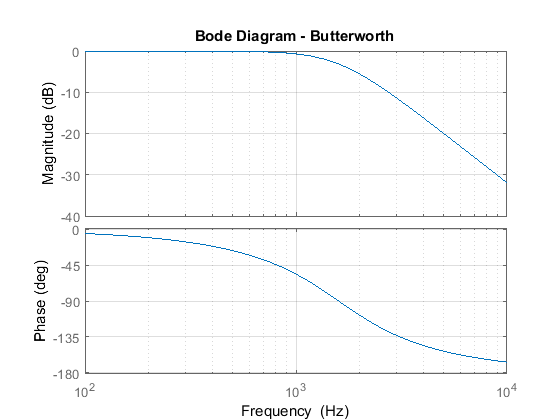
\includegraphics[width=0.3\linewidth]{Bilder/TP_Butterworth}
\caption{}
\label{fig:TP_Butterworth}
\end{figure}

\begin{figure}[h]
\centering
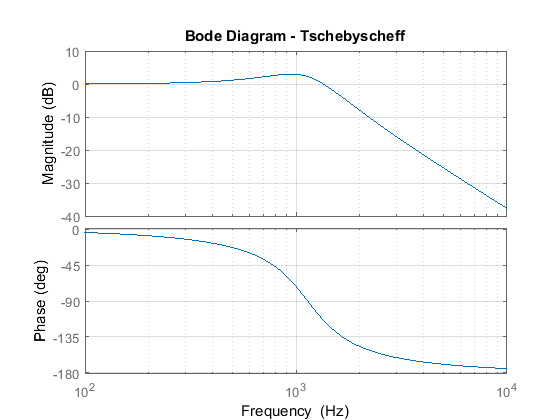
\includegraphics[width=0.3\linewidth]{Bilder/TP_Tschebyscheff}
\caption{}
\label{fig:TP_Tschebyscheff}
\end{figure}

\begin{figure}[h]
\centering
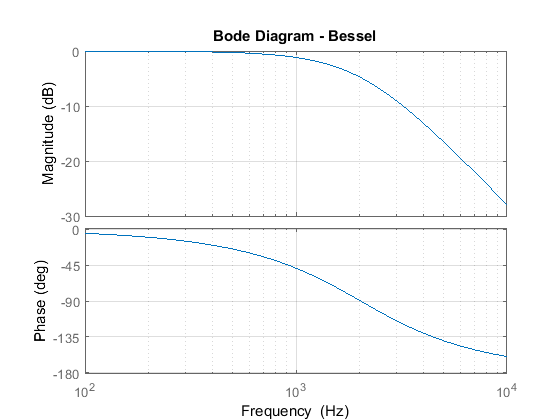
\includegraphics[width=0.3\linewidth]{Bilder/TP_Bessel}
\caption{}
\label{fig:TP_Bessel}
\end{figure}

\newpage


\subsubsection{Hochpassfilter}

In der Versuchsbeschreibung \cite{Aufgabenstellung} Kapitel 7: Gleichungen zum Universal-Filter wird die Übertragungsfunktion $H_{HP}$ angegeben mit.\\

\begin{alignat}{2}
H_{HP} (j \omega)&= \frac{U_{HP}}{U_{e}} &= \frac{R_{b} \cdot R_{d}}{R_{a} \cdot R_{c}} \cdot \frac{ \frac{R_{f} }{R_{d}} \cdot \left( j \omega \tau \right)^2 }{1+\frac{R_{b} \cdot R_{f}}{R_{c} \cdot R_{e}} \cdot  \left(j \omega \tau \right) + \frac{R_{f}}{R_{d}} \cdot \left ( j \omega \tau \right)^2}~~~~ mit ~\tau = R \cdot C
\end{alignat}

\noindent Durch die Wahl von $R_{b} = R_{c} = R_{d} = R_{0}$ vereinfacht sich die Gleichung zu:

\begin{alignat}{2}
H_{HP} (j \omega) &= \frac{R_{0}}{R_{a}} \cdot \frac{ 	\frac{R_{f} }{R_{d}} \cdot \left( j \omega \tau \right)^2 }	 {1+\frac{R_{f} \cdot R_{0}}{R_{0} \cdot R_{e}} \cdot  \left(j \omega \tau \right) + \frac{R_{f}}{R_{0}} \cdot \left ( j \omega \tau \right)^2}
\end{alignat}

\noindent Aus der Allgemeinen Gleichung eines Hochpassfilter 2. Ordnung können so die Parameter $a_{1}, b_{1}~und~V_{0}$ zugewiesen werden. $V_{\infty}$ ist die maximale Verstärkung bei $\omega -> \infty$.

\begin{alignat}{2}
V_{\infty} \cdot \frac{ \frac{1}{b_{1}} \cdot (j \omega)^2}{1 + \frac{a_{1}}{b_{1}} \cdot j \omega + \frac{1}{b_{1}} \cdot \left ( j \omega \right)^2} &= \frac{R_{0}}{R_{a}} \cdot \frac{ \frac{R_{f} }{R_{0}} \cdot \left( j \omega \tau \right)^2  }{1+\frac{R_{f} \cdot R_{0}}{R_{0} \cdot R_{e}} \cdot  \left(j \omega \tau \right) + \frac{R_{0}}{R_{d}} \cdot \left ( j \omega \tau \right)^2}
\end{alignat}

\begin{alignat}{2}
V_{\infty} &= \frac{R_{0}}{R_{a}}\\
b_{1} &= \frac{R_{0}}{R_{f}} \cdot \frac{1}{\tau^2}\\
\frac{a_{1}}{b_{1}} &= \frac{R_{f} \cdot R_{0}}{R_{0} \cdot R_{e}} \cdot \tau\\
a_{1} &= \frac{R_{f} \cdot R_{0}}{R_{0} \cdot R_{e} } \cdot \tau \cdot b_{1}\\
&\Rightarrow \frac{R_{f} \cdot R_{0}}{R_{0} \cdot R_{e} } \cdot \tau \cdot \frac{R_{0}}{R_{f}} \cdot \frac{1}{\tau^2}\\
&\Rightarrow \frac{R_{0}}{R_{e}} \cdot \frac{1}{\tau}
\end{alignat}

\newpage

\noindent \textbf{Allgemeine Formel zur Bestimmung der Grenzfrequenzen}\\\\

\noindent Der Amplitudengang lautet:

\begin{alignat}{2}
\lvert H_{HP (j \omega)} \rvert = \frac{\lvert V_{\infty} \rvert \cdot \left(\frac{1}{b_{1}} \right) \cdot \omega^2}{\sqrt{\left(1 - \left(\frac{1}{b_{1}} \right) \cdot \omega^2 \right)^2 + \left(\frac{a_{1}}{b_{1}} \right) \cdot \omega^2}}
\end{alignat}

\noindent Mit der Definition $H_{HP (j \omega_{g})} = \lvert H_{HP (j \omega)} \rvert_{max} \cdot \frac{1}{\sqrt{2}}$ und $V_{\infty} = 1$ (Tabelle \ref{tab:Tiefpaesse_Grundverstaerkung}) kann die Gleichung nach $\omega_{g}$ aufgelöst werden.

\begin{alignat}{2}
\frac{1}{\sqrt{2}} = \frac{\lvert V_{\infty} \rvert \cdot \left(\frac{1}{b_{1}} \right) \cdot \omega^2}{\sqrt{\left(1 - \left(\frac{1}{b_{1}} \right) \cdot \omega^2 \right)^2 + \left(\frac{a_{1}}{b_{1}} \right) \cdot \omega^2}}\\
\sqrt{2} \cdot \lvert V_{\infty} \rvert \cdot \left(\frac{1}{b_{1}} \right) \cdot \omega^2 = \sqrt{\left(1 - \left(\frac{1}{b_{1}} \right) \cdot \omega^2 \right)^2 + \left(\frac{a_{1}}{b_{1}} \right) \cdot \omega^2}\\
2 \cdot \lvert V_{\infty} \rvert^2 \cdot \left(\frac{1}{b_{1}^2} \right) \cdot \omega^2 = \left(1 - \left(\frac{1}{b_{1}} \right) \cdot \omega^2 \right)^2 + \left(\frac{a_{1}}{b_{1}} \right) \cdot \omega^2\\
0 = \left( \frac{1}{b_{1}^2} - 2 \cdot \lvert V_{\infty} \rvert^2 \cdot \frac{1}{b_{1}^2} \right) \cdot \omega^4 + \left(\frac{a_{1}^2}{b_{1}^2} - 2 \cdot \frac{1}{b_{1}} \right) \cdot \omega^2 + 1
\end{alignat}




\begin{alignat}{2}
0 = x^2 + \frac{a_{1}^2 - 2 \cdot b_{1}}{1 - 2 \cdot \lvert V_{\infty} \rvert^2} \cdot x + \frac{b_{1}^2}{1 - 2 \cdot \lvert V_{\infty} \rvert^2}
\end{alignat}

\noindent Bestimmen der Möglichen Frequenzen:

\begin{alignat}{2}
x_{1,2} &= -\frac{p}{2} \pm \sqrt{\frac{p}{2}^2 - q}\\
w_{g1} &= +\sqrt{x1}\\
w_{g2} &= -\sqrt{x1}\\
w_{g3} &= +\sqrt{x1}\\
w_{g4} &= -\sqrt{x2}
\end{alignat}

\newpage

\begin{table}[h]
	\centering
	\begin{tabular}{c|c|c}
		$HP_{Filtercharakteristik}$ & Grundverstärkung $V_{\infty}$	& Grenzfrequenz $f_{g}$	\\
		\hline
		\hline
		Butterworth	& 1	& 1,6107 kHz	\\
		Tschebyscheff	& 1	& 1,6055 kHz	\\
		Bessel	& 1	& 1,582 kHz 	\\
	\end{tabular}
	\caption{Hochpassfilter - Grundverstärkung $V_{\infty}$, Grenzfrequenz $f_{g}$ }
	\label{tab:Hochpaesse_Grundverstaerkung}
\end{table}

\textbf{Bodeplot der HP-Filter Butterworth, Tschebyscheff und Bessel.}

\begin{figure}[h]
	\centering
	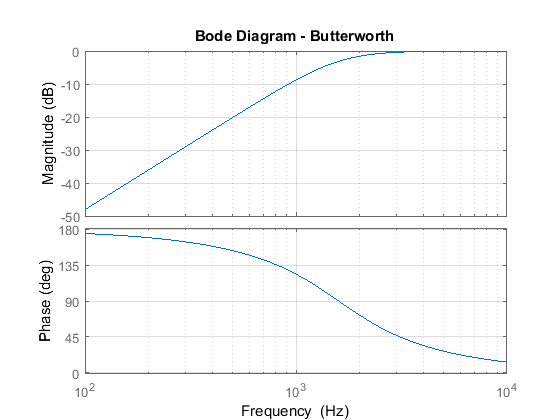
\includegraphics[width=0.3\linewidth]{Bilder/HP_Butterworth}
	\caption{}
	\label{fig:HP_Butterworth}
\end{figure}

\begin{figure}[h]
	\centering
	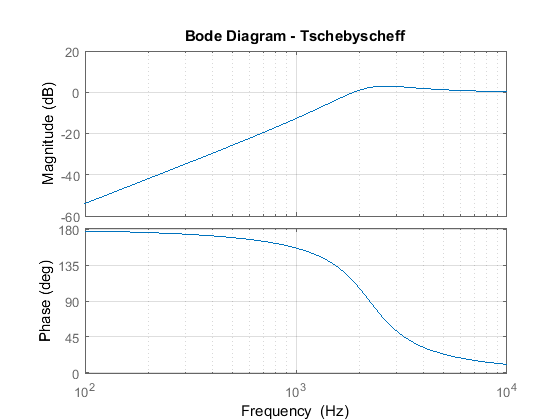
\includegraphics[width=0.3\linewidth]{Bilder/HP_Tschebyscheff}
	\caption{}
	\label{fig:HP_Tschebyscheff}
\end{figure}

\begin{figure}[h]
	\centering
	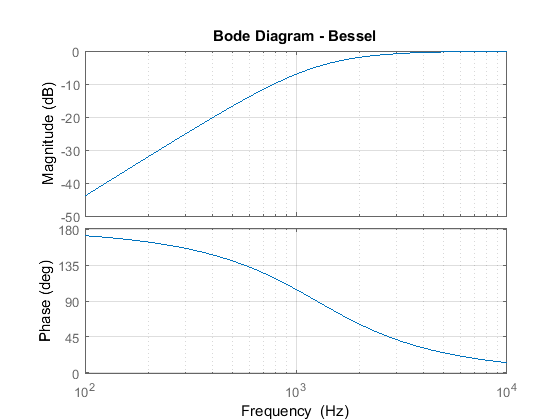
\includegraphics[width=0.3\linewidth]{Bilder/HP_Bessel}
	\caption{}
	\label{fig:HP_Bessel}
\end{figure}
	\section{Messungen}
\subsection{Verwendete Geräte}


\newpage

\subsection{Messung von Amplituden- und Phasengang der Filterschaltungen}
\noindent In diesem Versuch geht es darum, die Amplituden und Phasengänge der Butterworth-, Tschebyscheff- und Bessel-Tiefpässe und die Amplitudengänge der Butterworth-, Tschebyscheff- und Bessel-Hochpässe sowie des Bandpasses und der Bandsperre mittels dem Audio-Analyzer UVP zu messen. Die folgende Tabelle zeigt unsere gemessenen Grenzfrequenzen der Tiefpässe/Hochpässe. Die Graphen sind im Anhang zu finden.

	\begin{table}[h]
		\centering
		\begin{tabular}{c|c|c|c|c|c}
			$ $        & $Butterworth$ & $Tschebyscheff$ & $Bessel$  \\
			\hline
			$Tiefpass$ & $1.538kHz$    & $1.557kHz$      & $1.551kHz$  \\
			$Hochpass$ & $1.596kHz$    & $1.592kHz$      & $1.610kHz$  \\   
		\end{tabular}
		\caption{Gemessenen Grenzfrequenzen der verschieden Tiefpässe/Hochpässe}
		\label{tab:grenzfrequnzen_hp_tp}
	\end{table}
	
\noindent Anschließend ging es darum, die Phasengänge der oben genannten Filtertypen für den Tiefpass zu messen. Die Frequenzen bei einer Phasenverschiebung von $-60^\circ$ und $-120^\circ$ wurden bestimmt und in die folgende Tabelle eingetragen. Auch diese Graphen sind im Anhang zu finden.

\begin{table}[h]
	\centering
		\begin{tabular}{c|c|c|c|c|c}
			$ $           & $Butterworth$ & $Tschebyscheff$ & $Bessel$  \\
			\hline		
		    $-60^\circ $ & $1.046kHz$    & $898.250kHz$    & $1.229kHz$  \\
			$-120^\circ$ & $2.381kHz$    & $1.400kHz$      & $3.225kHz$  \\   
	\end{tabular}
	\caption{Frequenzen bei einer Phasenverschiebung von $-60^\circ$ und $-120^\circ$ }
	\label{tab:phasenverschiebung_hp_tp}
\end{table}
	
\noindent Schließlich wurden die Mittenfrequenz und Sperrfrequenz des Bandpasses sowie der Bandsperre gemessen. Ergebnisse sind der folgenden Tabelle zu entnehmen. Für die Graphen siehe Anhang.

\begin{table}[h]
	\centering
	\begin{tabular}{c|c|c|c|c|c}
		$ $          & $Mittenfrequenz$ & $Sperrfrequenz$  \\
		\hline
		$Bandpass$   & $1.556kHz$       & $/$         \\
		$Bandsperre$ & $/$              & $1.568kHz$  \\   
	\end{tabular}
	\caption{Mittenfrequenz und Sperrfrequenz des Bandpasses sowie der Bandsperre}
	\label{tab:grenzfrequnzen_bs_bp}
\end{table}

\newpage

\subsection{Sprungantworten der Tiefpässe}
\noindent In diesem Versuch geht darum, die Anstiegszeit, Überschwingen und die Einstiegszeit der drei Tiefpässe nach Butterworth, Tschebyscheff und Bessel aus der Sprungantwort zu bestimmen. Die Filter wurde mit einem Rechtecksignal ($500mV_pp$ und $250mv$ Offset und variabler Frequenz) angesteuert. Eingangs- und Ausgangssignal wurden in einem gemeinsamen Oszillogramm dargestellt. 

\begin{figure}[h]
\centering
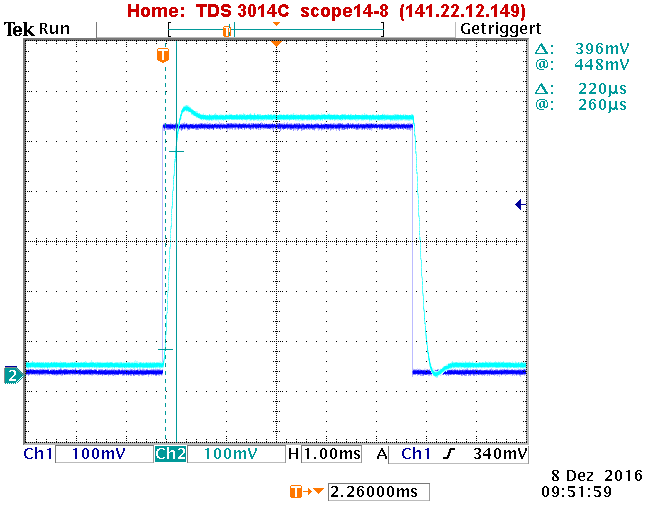
\includegraphics[width=0.7\linewidth]{Bilder/ImLabor/Sprungantwort_5_8_Butter_Anstiegszeit}
\caption{Sprungantwort Butterworth-Tiefpass}
\label{fig:Sprungantwort_5_8_Butter_Anstiegszeit}
\end{figure}

\begin{figure}[h]
\centering
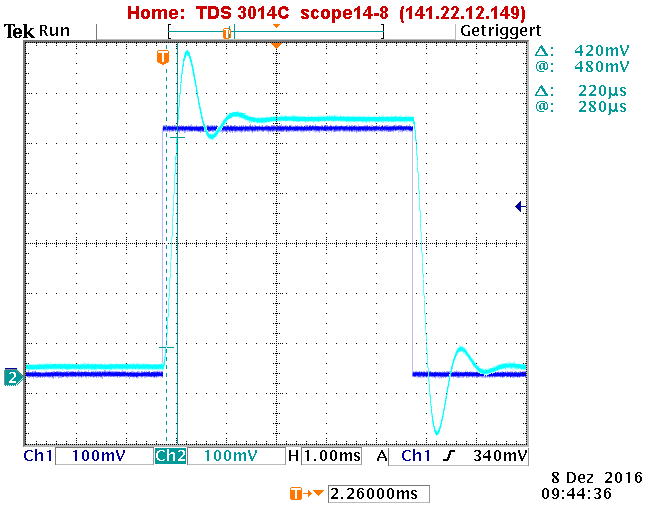
\includegraphics[width=0.7\linewidth]{Bilder/ImLabor/Sprungantwort_5_3_Tscheby_Anstiegszeit}
\caption{Sprungantwort Tschebyscheff-Tiefpass}
\label{fig:Sprungantwort_5_3_Tscheby_Anstiegszeit}
\end{figure}

\begin{figure}[h]
\centering
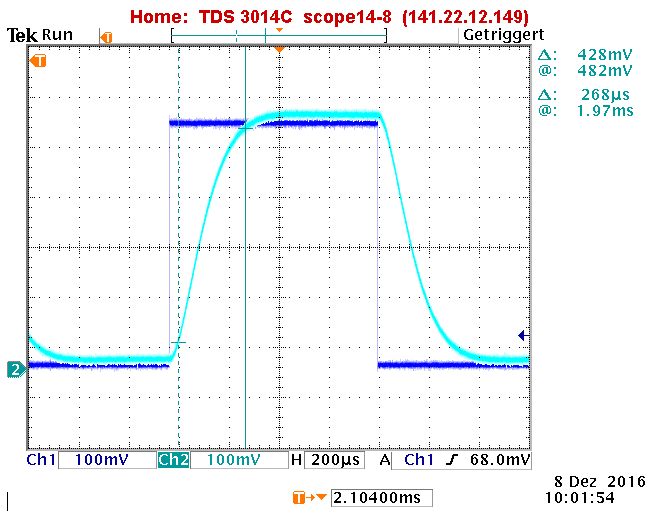
\includegraphics[width=0.7\linewidth]{Bilder/ImLabor/Sprungantwort_5_1_Bessel_Anstiegszeit}
\caption{Sprungantwort Bessel-Tiefpass}
\label{fig:Sprungantwort_5_1_Bessel_Anstiegszeit}
\end{figure}

\newpage
	\section{Auswertung}
\subsection{Zu: Messung von Amplituden- und Phasengang}
\subsubsection{Grenzfrequenzen Tiefpässe/Hochpässe}
\noindent Alle Messwerte der Grenzfrequenzen werden zusammen mit den vorausberechneten Werten in einer Tabelle dargestellt und verglichen.
   	  
   	  \begin{table}[h]
   	  	\centering
   	  	\begin{tabular}{c|c|c|c|c|c|}
						   	&	& $f_{g,rech}$	& $f_{g,mess}$	& $\Delta f_g$	& $\Delta f_g$ [\%] \\
   	  		\hline
   	  		Butterworth		& TP& $1.573kHz$	& $1.538kHz$	& $35Hz$		& $2,23$\\
							& HP& $1.611kHz$	& $1.596kHz$	& $15Hz$		& $0,93$\\
			\hline
   	  		Tschebyscheff	& TP& $1.578kHz$	& $1.557kHz$	& $21Hz$		& $1,33$\\
				   	  		& HP& $1.606kHz$	& $1.592kHz$	& $14Hz$		& $0,87$\\
   	  		\hline
   	  		Bessel			& TP& $1.585kHz$	& $1.551kHz$	& $34Hz$		& $2,15$\\
				   	  		& HP& $1.582kHz$	& $1.610kHz$	& $28Hz$		& $1,77$
   	  	\end{tabular}
		\caption{Vergleich der Werte, Tiefpässe und Hochpässe}
		\label{tab:grenzfrequnzen_hp_tp_vorausberechnung}
   	  \end{table}
   	  
   	  \noindent Geringe Messabweichungen ergeben sich zunächst aus dem Messgraphen des Audioanalyzers, da der Cursor nicht immer auf genau -3dB eingestellt werden kann, die Messpunkte des Messgeräts variieren. Zudem haben die verwendeten Widerstände nur idealer Weise die nominalen Werte, diese variieren auch. Mit Abweichungen von maximal $2,23$\% kann von einer relativ guten Messung ausgegangen werden.
   	  

\subsubsection{Mitten-/Sperrfrequenz, Bandpass und Bandsperre}
\noindent Die gemessenen Frequenzen werden zusammen mit den vorausberechneten Werten in einer Tabelle dargestellt und anschließend verglichen. Im folgenden wird $f_m$ die Mittenfrequenz sein und $f_s$ die Sperrfrequenz.

		\begin{table}[h]
			\centering
			\resizebox{\textwidth}{!}{
			\begin{tabular}{c|c|c|c|c|c|c|c|c|}
							& $f_{m,rech}$	& $f_{m,mess}$	& $\Delta f_m$	& $\Delta f_m$ [\%]	& $f_{s,rech}$	& $f_{s,mess}$	& $\Delta f_s$	& $\Delta f_s$ [\%]\\
				\hline
				Bandpass	& $1.556kHz$	& $1.591kHz$	& $35Hz$		& $2,25$			& - 			& - 			& - 		& - \\
				\hline
				Bandsperre	& -				& -				& - 			& - 				& $1.568kHz$	& $1.592kHz$	& $24Hz$ & $1,53$\\   
			\end{tabular}
			}
			\caption{Vergleich der Werte, Bandpass und Bandsperre}
			\label{tab:grenzfrequnzen_bs_bp_vorausberechnung}
		\end{table}
		
		\noindent Auch hier ergeben sich die geringen Abweichungen durch die zuvor beschriebenen Umstände.
		
\newpage

\subsubsection{Gemessenen Frequenzen bei einer Phasenverschiebung}
\noindent Die gemessenen Frequenzen bei gewählten Phasenverschiebungen werden in einer Tabelle dargestellt und anschließend mit den errechneten Werten verglichen. Die folgenden Messungen beziehen sich auf die Tiefpässe der jeweiligen Arten.

		\begin{table}[h]
			\centering
			\begin{tabular}{c|c|c|}
								& $f_{mess,-60^\circ}$	& $f_{mess,-120^\circ}$	\\
				\hline		
				Butterworth		& $1.046kHz$			& $2.381kHz$		\\
				\hline
				Tschebyscheff	& $898.250kHz$			& $1.400kHz$		\\ 
				\hline
				Bessel			& $1.229kHz$			& $3.225kHz$		\\
			\end{tabular}
			\caption{Gemessene Frequenzen bei einer Phasenverschiebung von $-60^\circ$, $-120^\circ$}
			\label{tab:phasenverschiebung_tp_vorausberechnung_60_120}
		\end{table}
		
\noindent Aus den bei einer bestimmten Phasenverschiebung gemessenen Frequenzen ist es möglich die Koeffizienten der drei Filterarten zu bestimmen. 
\noindent Für einen Tiefpass bestimmter Art der 2. Ordnung gilt:

\small{
\begin{alignat*}{2}
arg\underline{H}_{TP}(\Omega) &= arg(V_0) - arctan(\frac{a_1 \cdot \Omega}{1-b_1\cdot \Omega^2}) \\
tan(arg\underline{H}_{TP}(\Omega)) &= tan(0) - \frac{a_1 \cdot \Omega}{1-b_1\cdot \Omega^2}\\
a_1 &= \frac{\Bigl(- tan(arg\underline{H}_{TP}(\Omega))\Bigr)\Bigl(1-b_1 \cdot \Omega^2\Bigr)}{\Omega}\\
\frac{\Bigl(- tan(arg\underline{H}_{TP}(\Omega_{-60^\circ}))\Bigr)\Bigl(1-b_1 \cdot \Omega_{-60^\circ}^2\Bigr)}{\Omega_{-60^\circ}} &= \frac{\Bigl(- tan(arg\underline{H}_{TP}(\Omega_{-120^\circ}))\Bigr)\Bigl(1-b_1 \cdot \Omega_{-120^\circ}^2\Bigr)}{\Omega_{-120^\circ}}\\
\frac{\Bigl(- tan(-60^\circ))\Bigr)\Bigl(1-b_1 \cdot \Omega_{-60^\circ}^2\Bigr)}{\Omega_{-60^\circ}} &= \frac{\Bigl(- tan(-120^\circ)\Bigr)\Bigl(1-b_1 \cdot \Omega_{-120^\circ}^2\Bigr)}{\Omega_{-120^\circ}}\\
\frac{\Bigl( \sqrt{3} \Bigr)\Bigl(1-b_1 \cdot \Omega_{-60^\circ}^2\Bigr)}{\Omega_{-60^\circ}} &= \frac{\Bigl(-\sqrt{3}\Bigr)\Bigl(1-b_1 \cdot \Omega_{-120^\circ}^2\Bigr)}{\Omega_{-120^\circ}}\\
\rightarrow b_1 &= \frac{\sqrt{3}\cdot \Omega_{-120^\circ}+\sqrt{3}\cdot \Omega_{-60^\circ}}
{\sqrt{3}\cdot \Omega_{-120^\circ}\cdot \Omega_{-60^\circ}^2 +\sqrt{3}\cdot \Omega_{-60^\circ}\cdot \Omega_{-120^\circ}^2}
\end{alignat*}}

\newpage

\noindent Anschließend es ist möglich mit einer gegebenen Frequenz und $b_1$ den Koeffizienten $a_1$ zu berechnen:

\small{
	\begin{alignat*}{2}
	arg\underline{H}_{TP}(\Omega) &= arg(V_0) - arctan(\frac{a_1 \cdot \Omega}{1-b_1\cdot \Omega^2}) \\
	tan(arg\underline{H}_{TP}(\Omega)) &= tan(0) - \frac{a_1 \cdot \Omega}{1-b_1\cdot \Omega^2}\\
	\rightarrow a_1 &= \frac{\Bigl(- tan(arg\underline{H}_{TP}(\Omega))\Bigr)\Bigl(1-b_1 \cdot \Omega^2\Bigr)}{\Omega}\\
	\end{alignat*}}

\noindent Aus den Berechnungen ergeben sich folgende Ergebnisse: \\

	\begin{table}[h]
		\centering
		\begin{tabular}{c|c|c|c||c|c|c}
			$ $             & $ a_{1, errechnet} $ & $ a_{1, ideal} $ & $\Delta a_1$ [\%] 
							& $b_{1, errechnet} $ & $ b_{1, ideal} $ & $\Delta b_1$ [\%] \\
			\hline	
			$Butterworth$   & $1.4279$             & $1.414$          & $0.98$            
			                & $0.9498$             & $1$              & $5.02$  \\ 	  	
			\hline
			$Tschebyscheff$ & $1.076$              & $1.065$          & $1.03$ 
			                & $1.928$              & $1.931$          & $0.16$  \\  
			\hline
			$ Bessel$ 		& $1.353$	           & $1.362$          & $0.66$  
			                & $0.607$              & $0.618$		  & $1.78$
		\end{tabular}
		\caption{Gegenüberstellung: errechnete und ideale Koeffizienten }
		\label{tab:koeffizienten}
	\end{table}
	
\newpage

\subsection{Zu: Sprungantworten der Tiefpässe}
\noindent Die Anstiegszeit, das Überschwingen sowie die Einschwingzeit der drei Tiefpässe wurden gemeinsam in einer Tabelle zusammengefasst und verglichen.

\begin{table}[h]
	\centering
	\begin{tabular}{c|c|c|c|c|c}
						& Anstiegszeit 	& Überschwingen	& Einschwingzeit  \\
		\hline
		Butterworth		& $220\mu s$	& $4.86\%$		& $320\mu s$ \\
		\hline
		Tschebyscheff	& $220\mu s$	& $27.24\%$		& $1.06ms$   \\
		\hline
		Bessel			& $268\mu s$	& $0\%$			& $308\mu s$ \\
	\end{tabular}
	\caption{Anstiegszeit, Überschwingen und Einschwingzeit der drei Tiefpässe}
	\label{tab:sprungantworten_tp}
\end{table}

\noindent Die Werte wurden den Oszillogrammen entnommen. Diese sind im Anhang zu finden.

\noindent In Tabelle \ref{tab:sprungantworten_tp} fällt auf, dass bei dem Tschebyscheff Tiefpass ein relativ großer Überschwinger stattfindet. Werden die benutzten Widerstände überprüft, da diese die drei verschiedenen Schaltungen unterscheiden, kann erkannt werden, dass die Widerstände $R_a$, $R_b$, $R_c$ und $R_f$ bei jeder gleich bleiben. Der Widerstand $R_e$ ändert sich geringfügig und der Widerstand $R_d$ erfährt große Änderungen. Dadurch kann folgende Theorie aufgestellt werden: Wird der Widerstand $R_d$ erhöht, verringert sich das Überschwingen und wird dieser reduziert, erhöht sich das Überschwingen in der Sprungantwort. Diese Theorie kann mit einer Spice-Simulation bestätigt werden. Dadurch ist nun auch bekannt, dass sowie der Widerstand $R_e$ erhöht wird, das Überschwingen sich auch erhöht. Wird dieser reduziert, nimmt das Überschwingen auch ab.








	\section{Anhang}
\subsection{Amplitudengänge}
\subsubsection{Tiefpässe}

\begin{figure}[h]
\centering
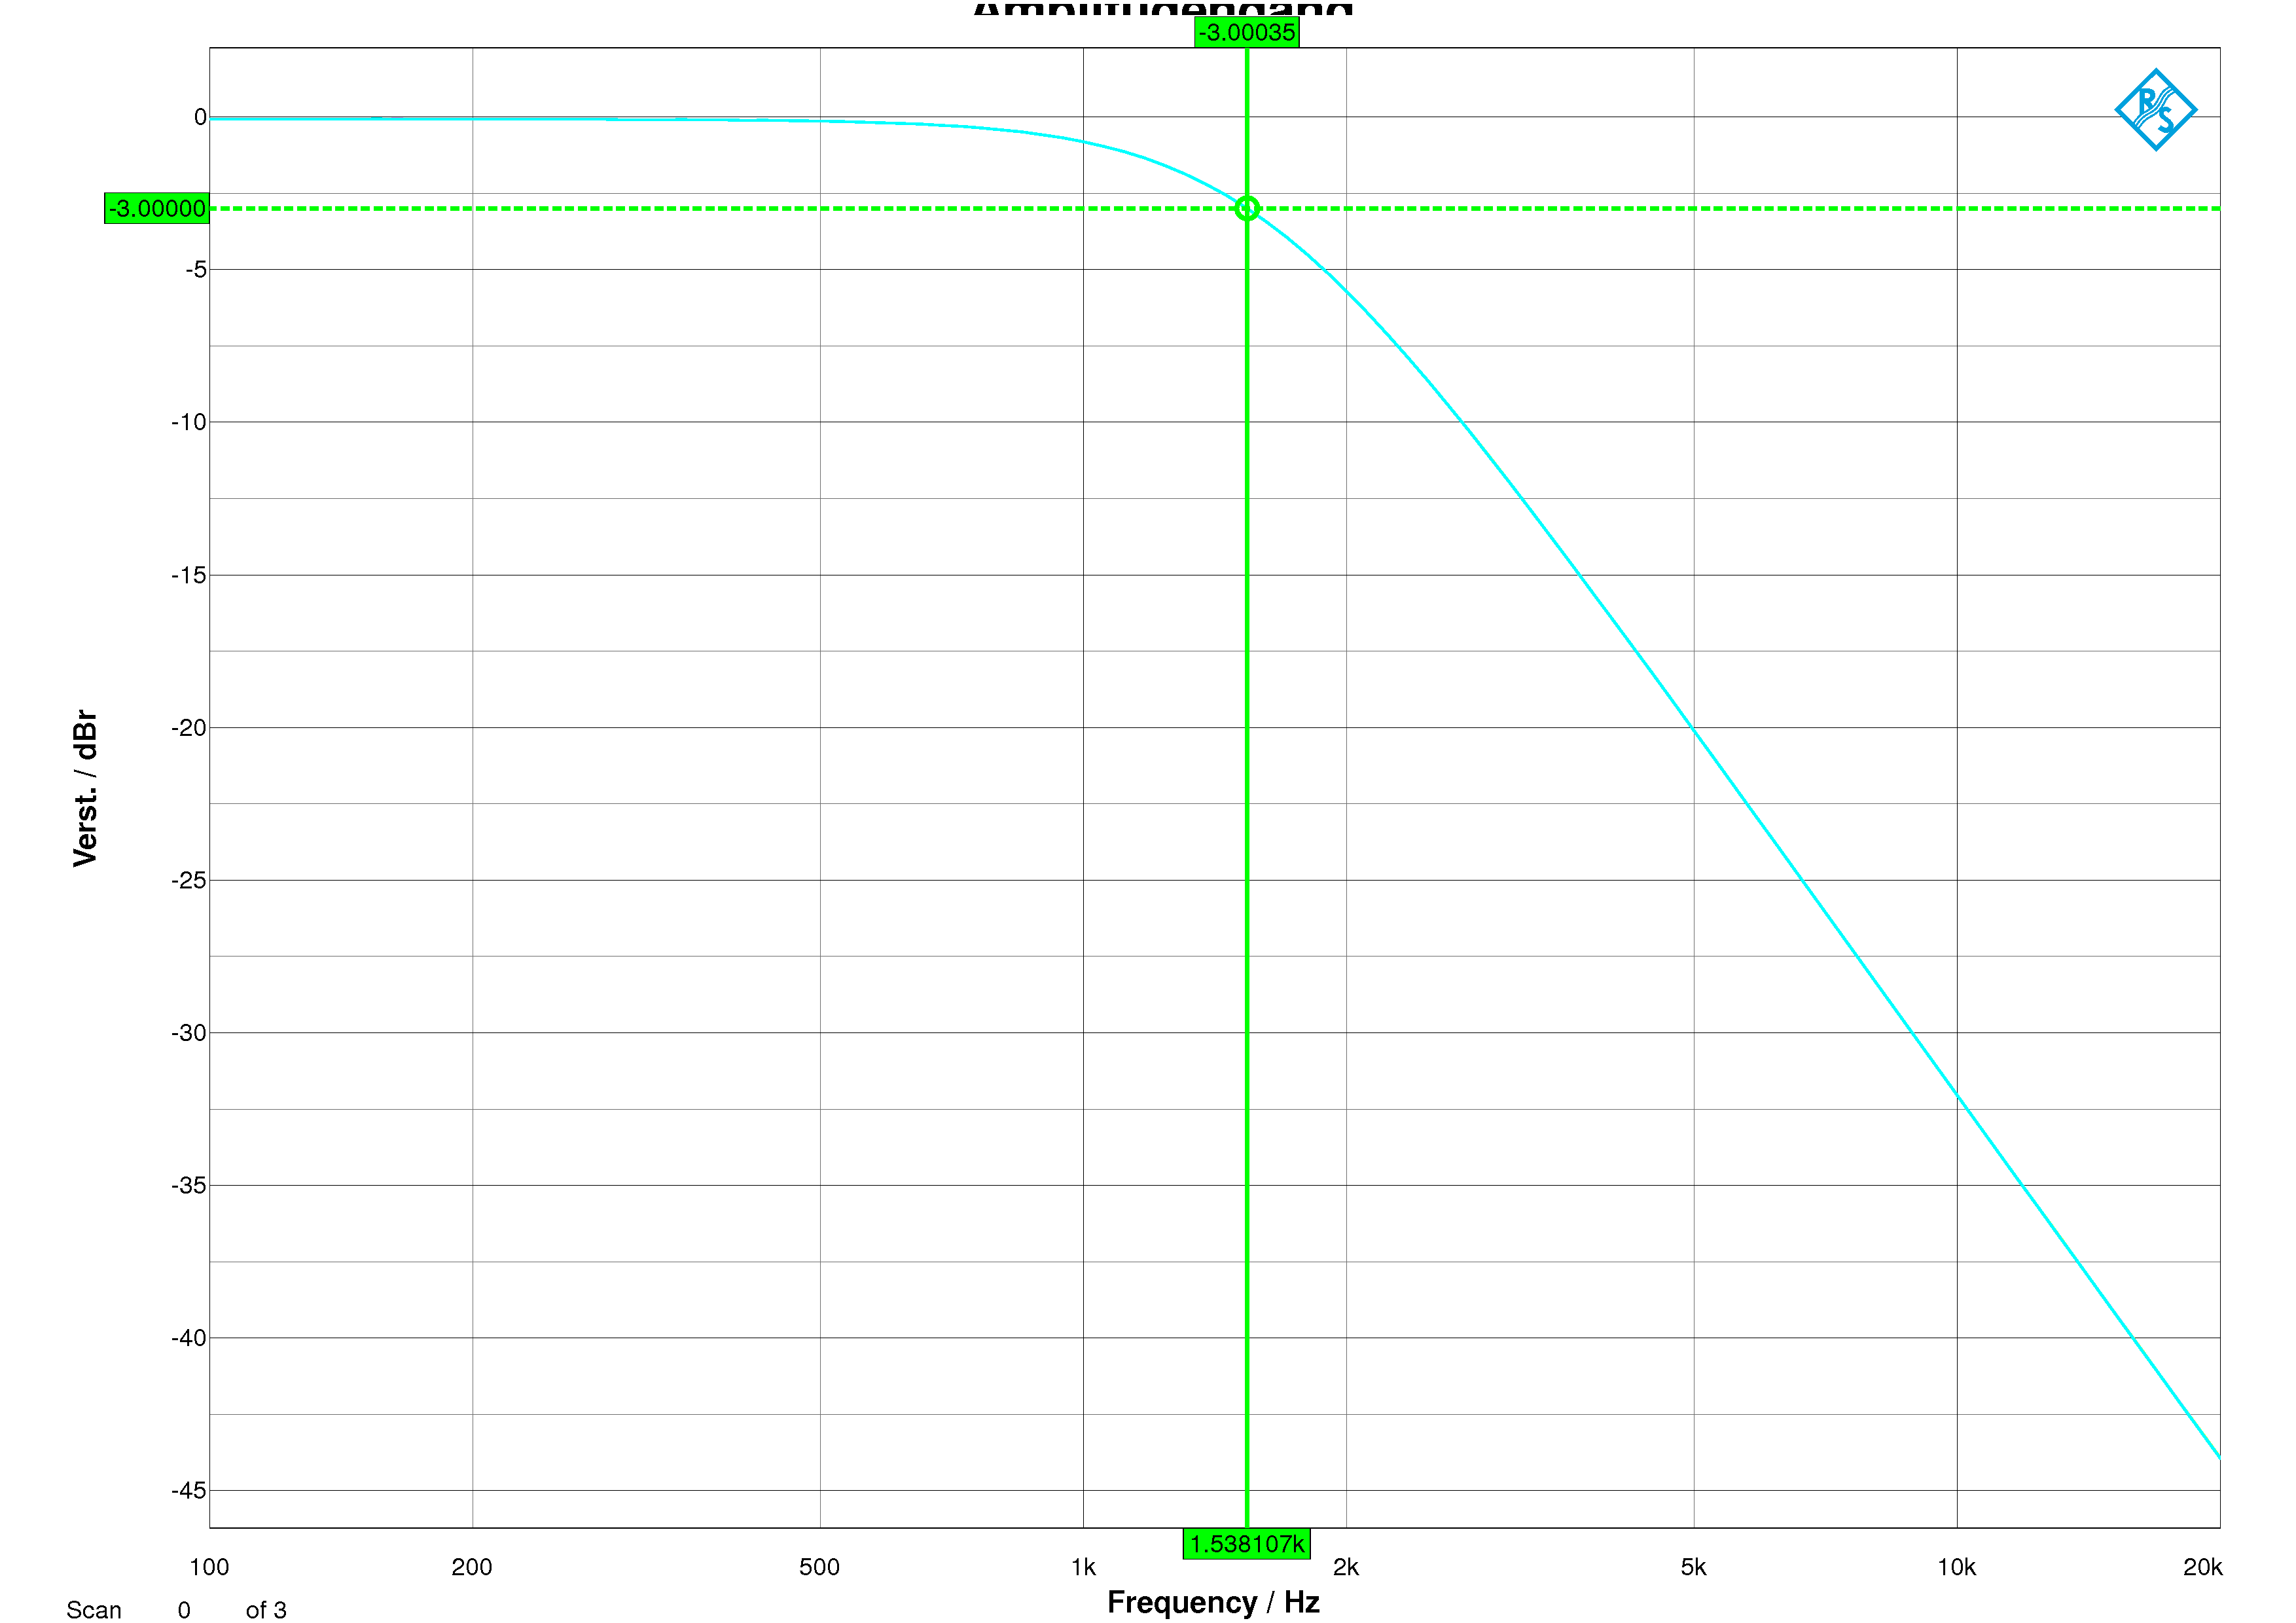
\includegraphics[width=0.60\linewidth]{Bilder/ImLabor/Amplitudengang_2_1_Butter_TP}
\caption{Amplitudengang Butterworth-Tiefpass mit Marker}
\label{fig:Amplitudengang_2_1_Butter_TP}
\end{figure}

\begin{figure}[h]
\centering
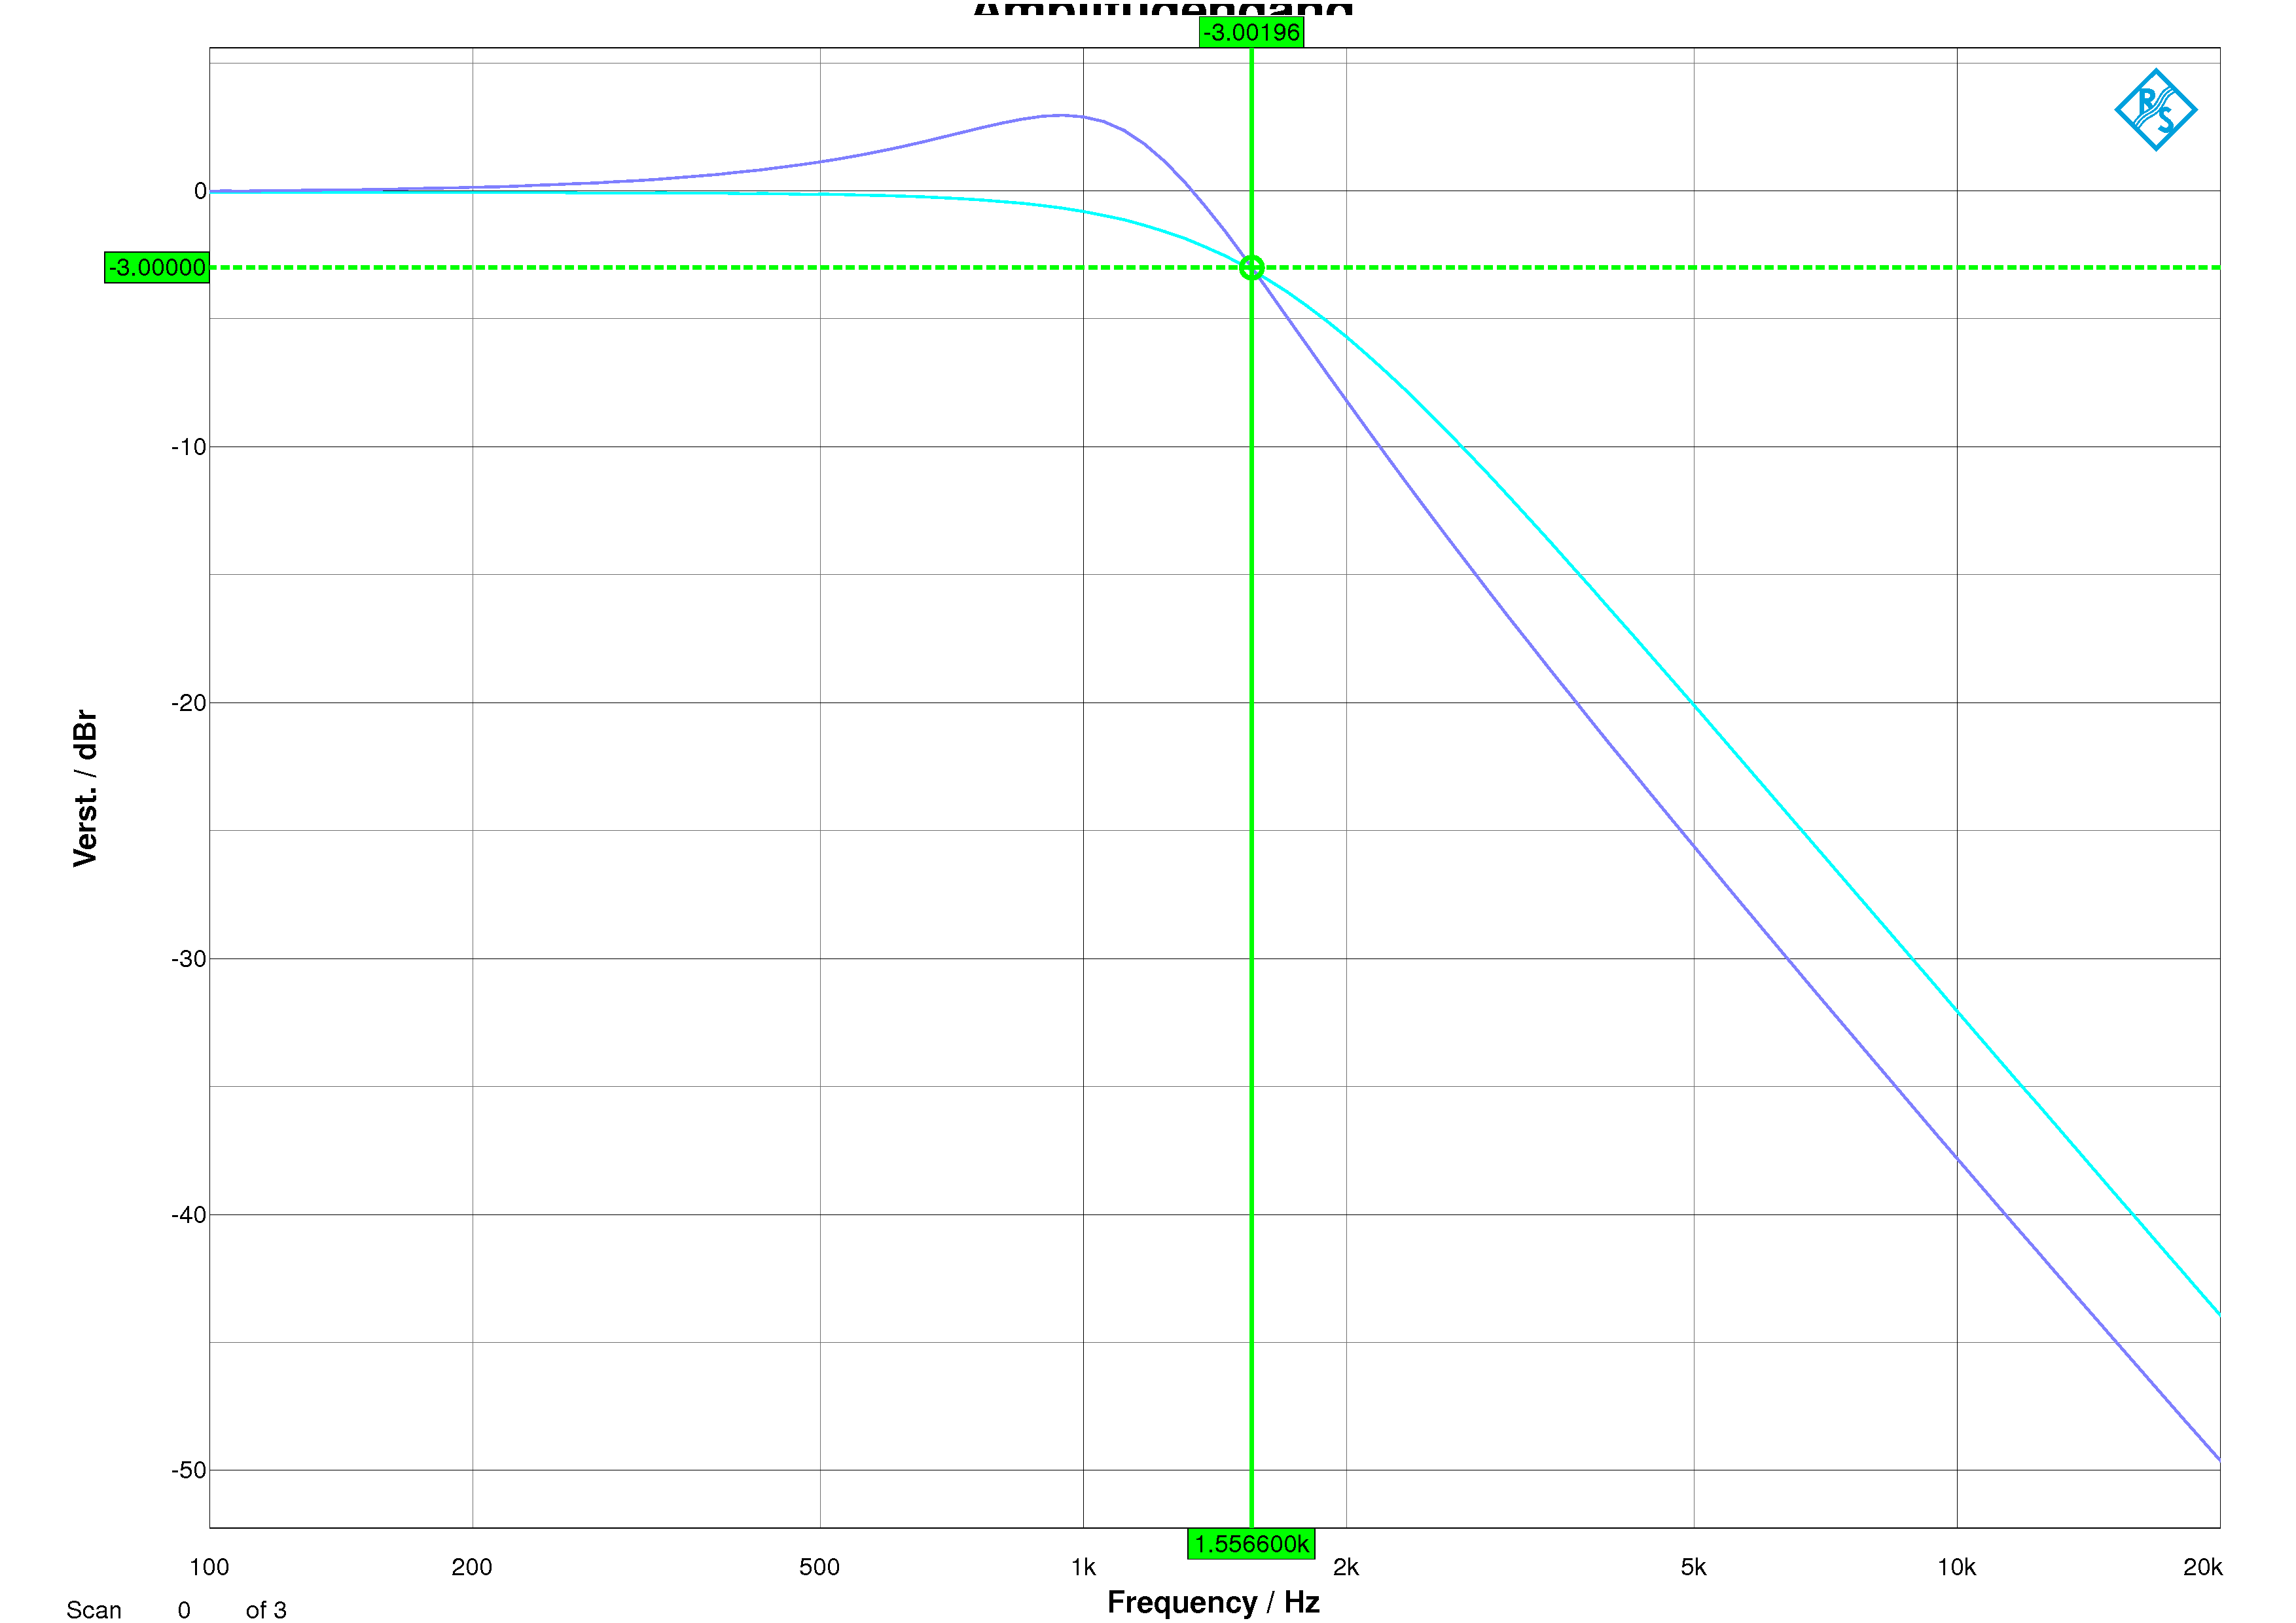
\includegraphics[width=0.60\linewidth]{Bilder/ImLabor/Amplitudengang_2_2_Tscheby_TP}
\caption{Amplitudengang Butterworth- und Tschebyscheff-Tiefpass mit Marker bei Tschebyscheff}
\label{fig:Amplitudengang_2_2_Tscheby_TP}
\end{figure}

\begin{figure}[h]
\centering
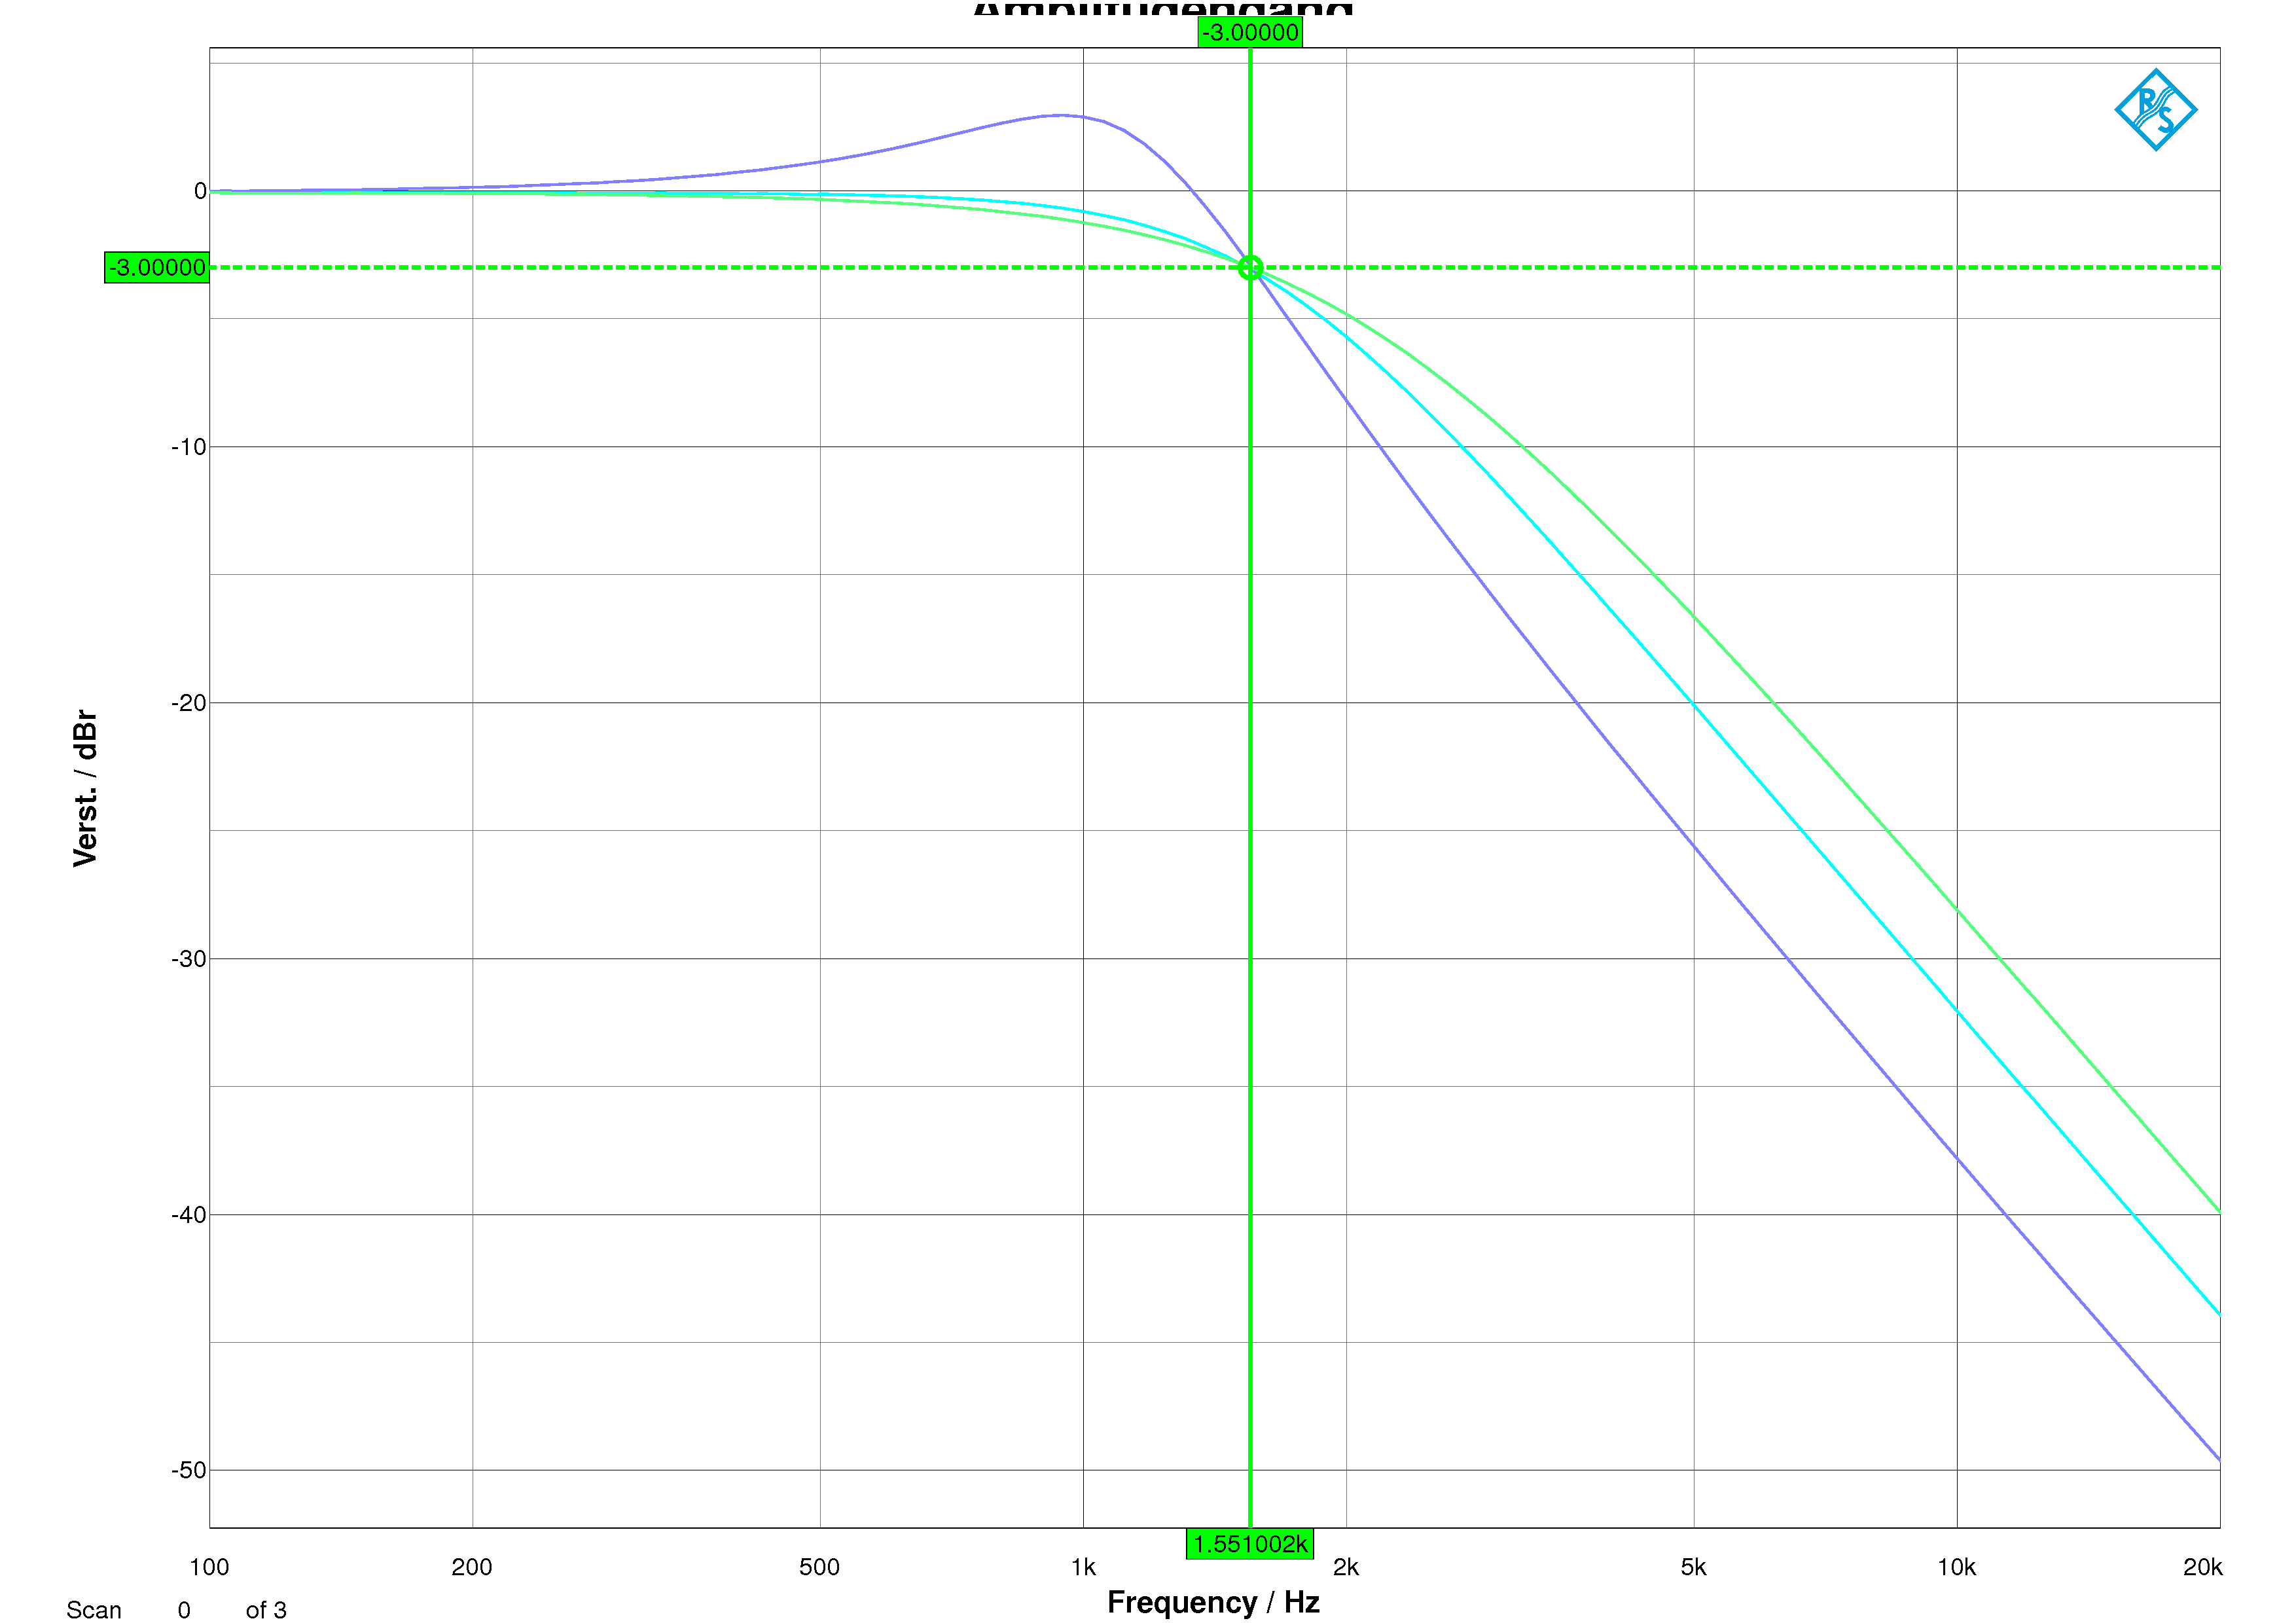
\includegraphics[width=0.60\linewidth]{Bilder/ImLabor/Amplitudengang_2_3_Bessel_TP_Alle}
\caption{Amplitudengang Butterworth-, Tschebyscheff- und Bessel-Tiefpass mit Marker bei Bessel}
\label{fig:Amplitudengang_2_3_Bessel_TP_Alle}
\end{figure}

\newpage
\newpage

\subsubsection{Hochpässe}

\begin{figure}[h]
\centering
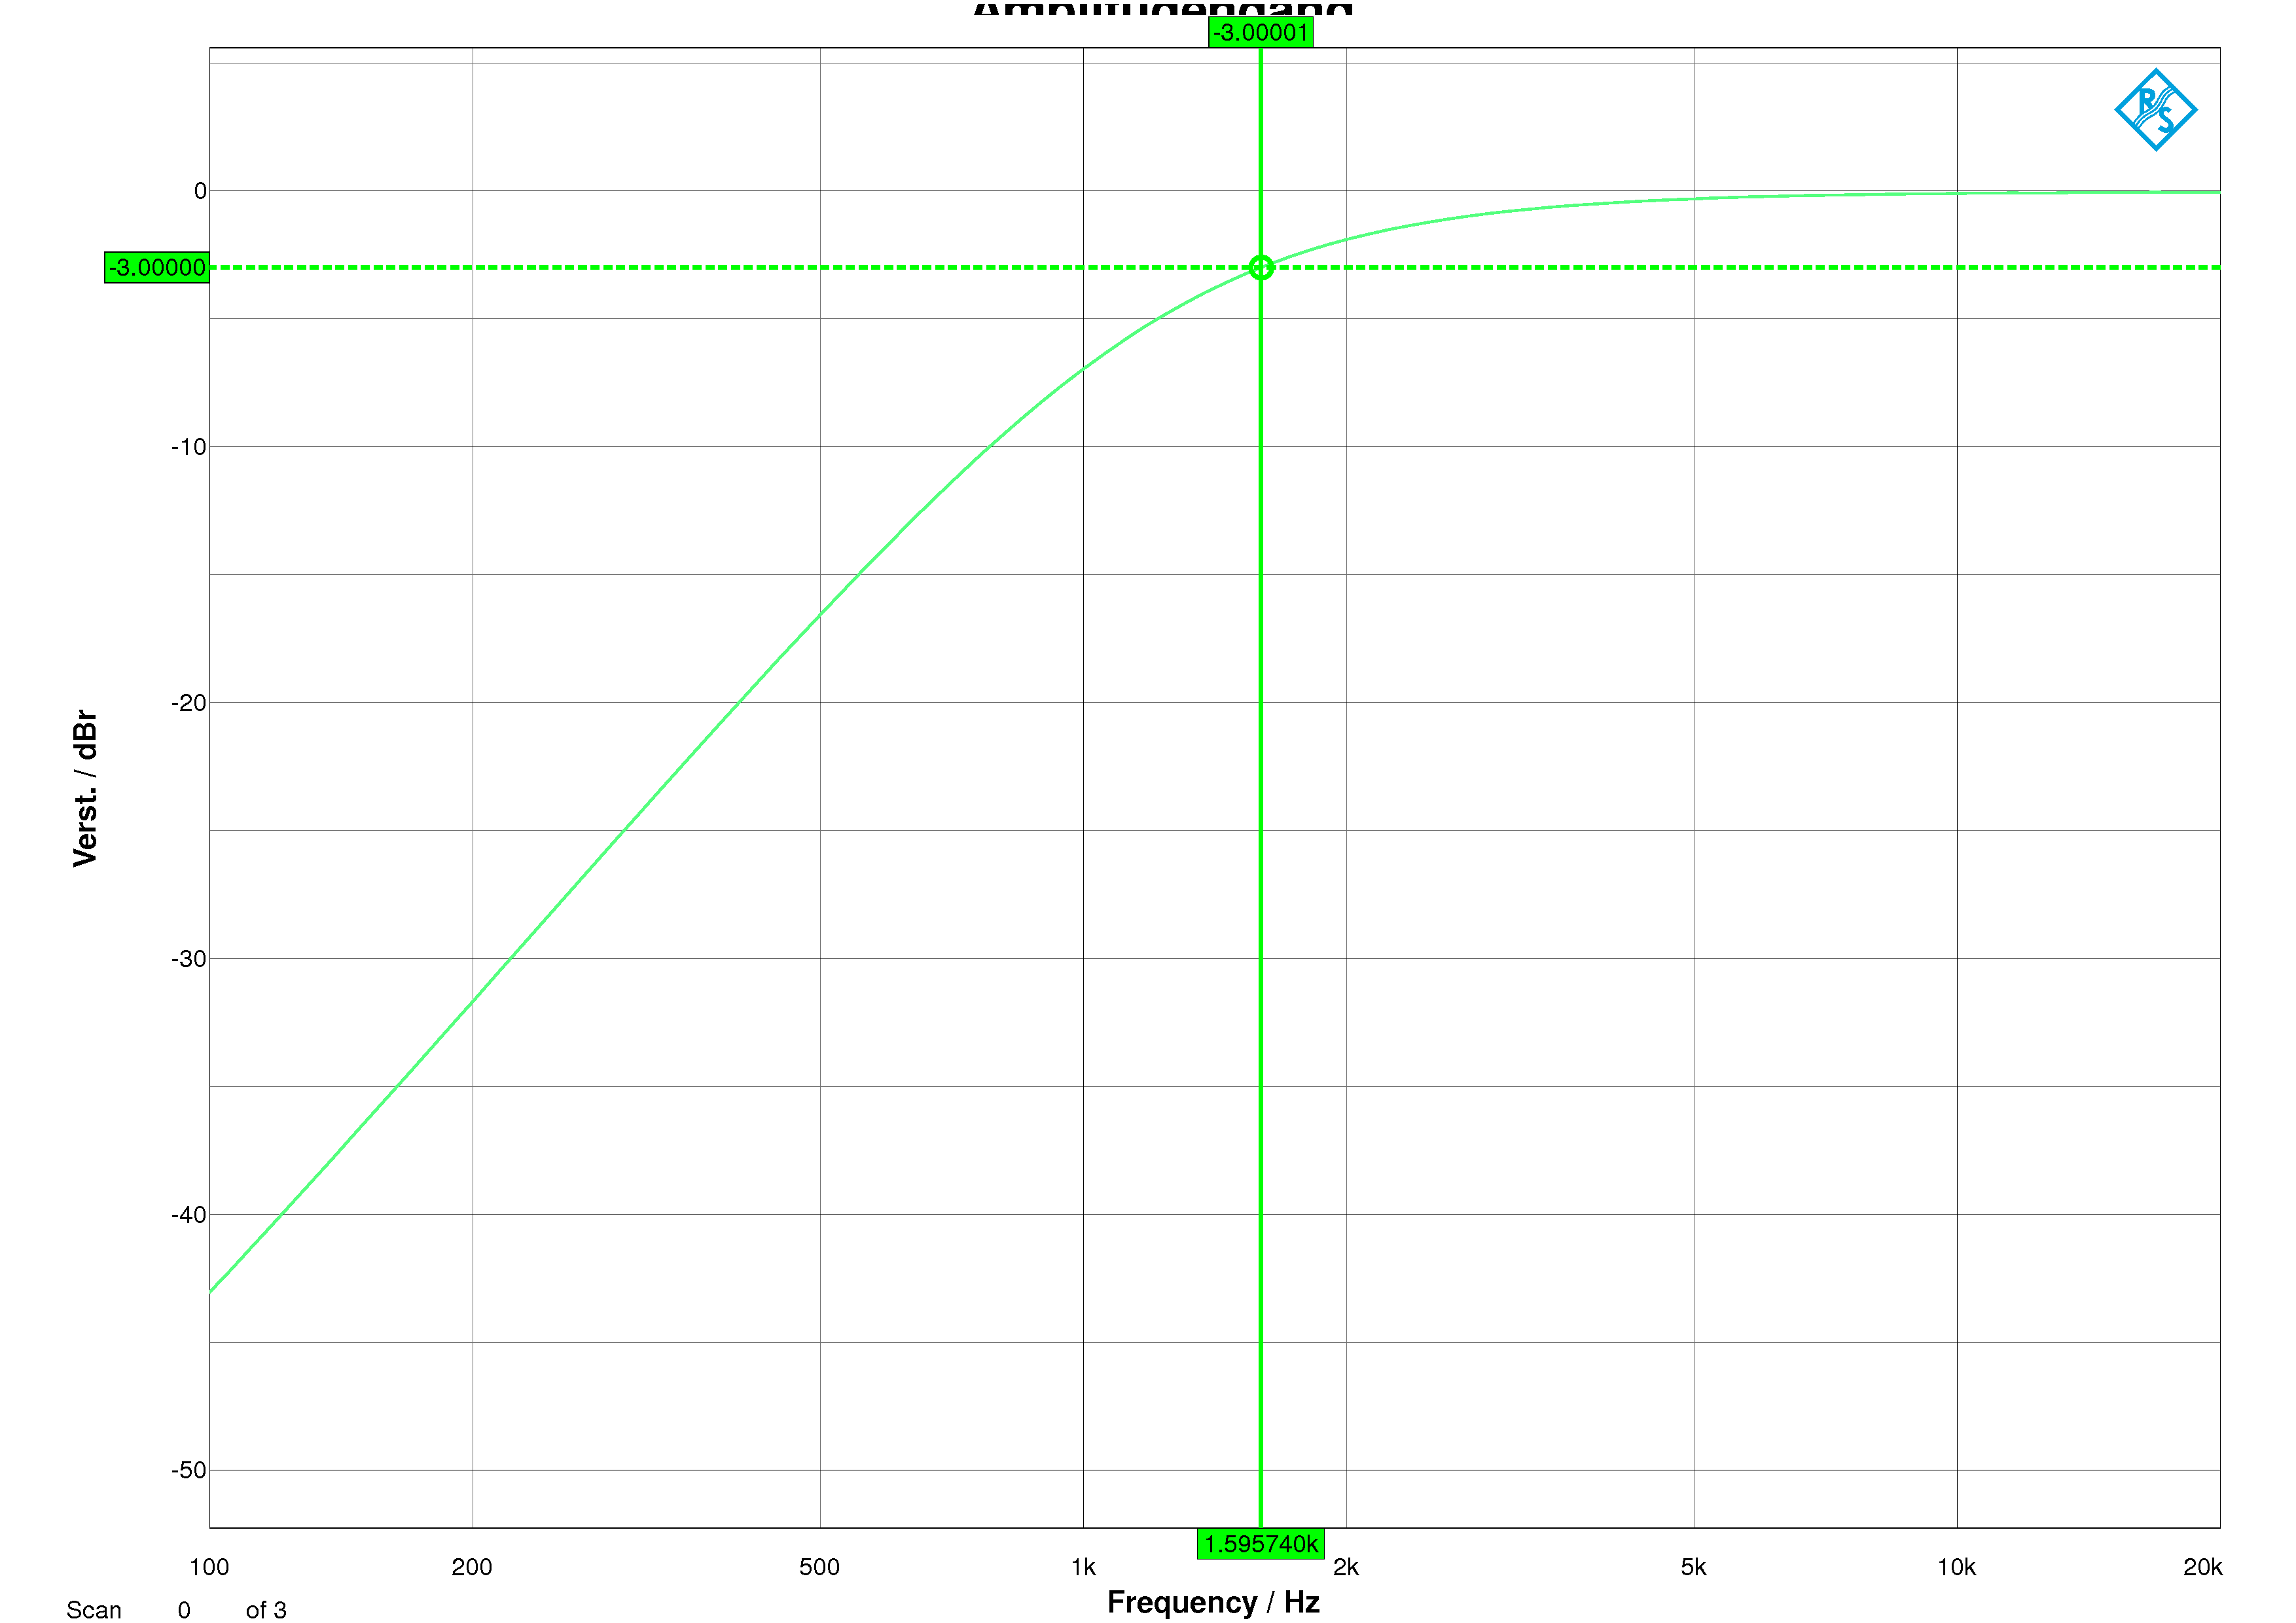
\includegraphics[width=0.60\linewidth]{Bilder/ImLabor/Amplitudengang_1_1_Butter_HP}
\caption{Amplitudengang Butterworth-Hochpass mit Marker}
\label{fig:Amplitudengang_1_1_Butter_HP}
\end{figure}

\begin{figure}[h]
\centering
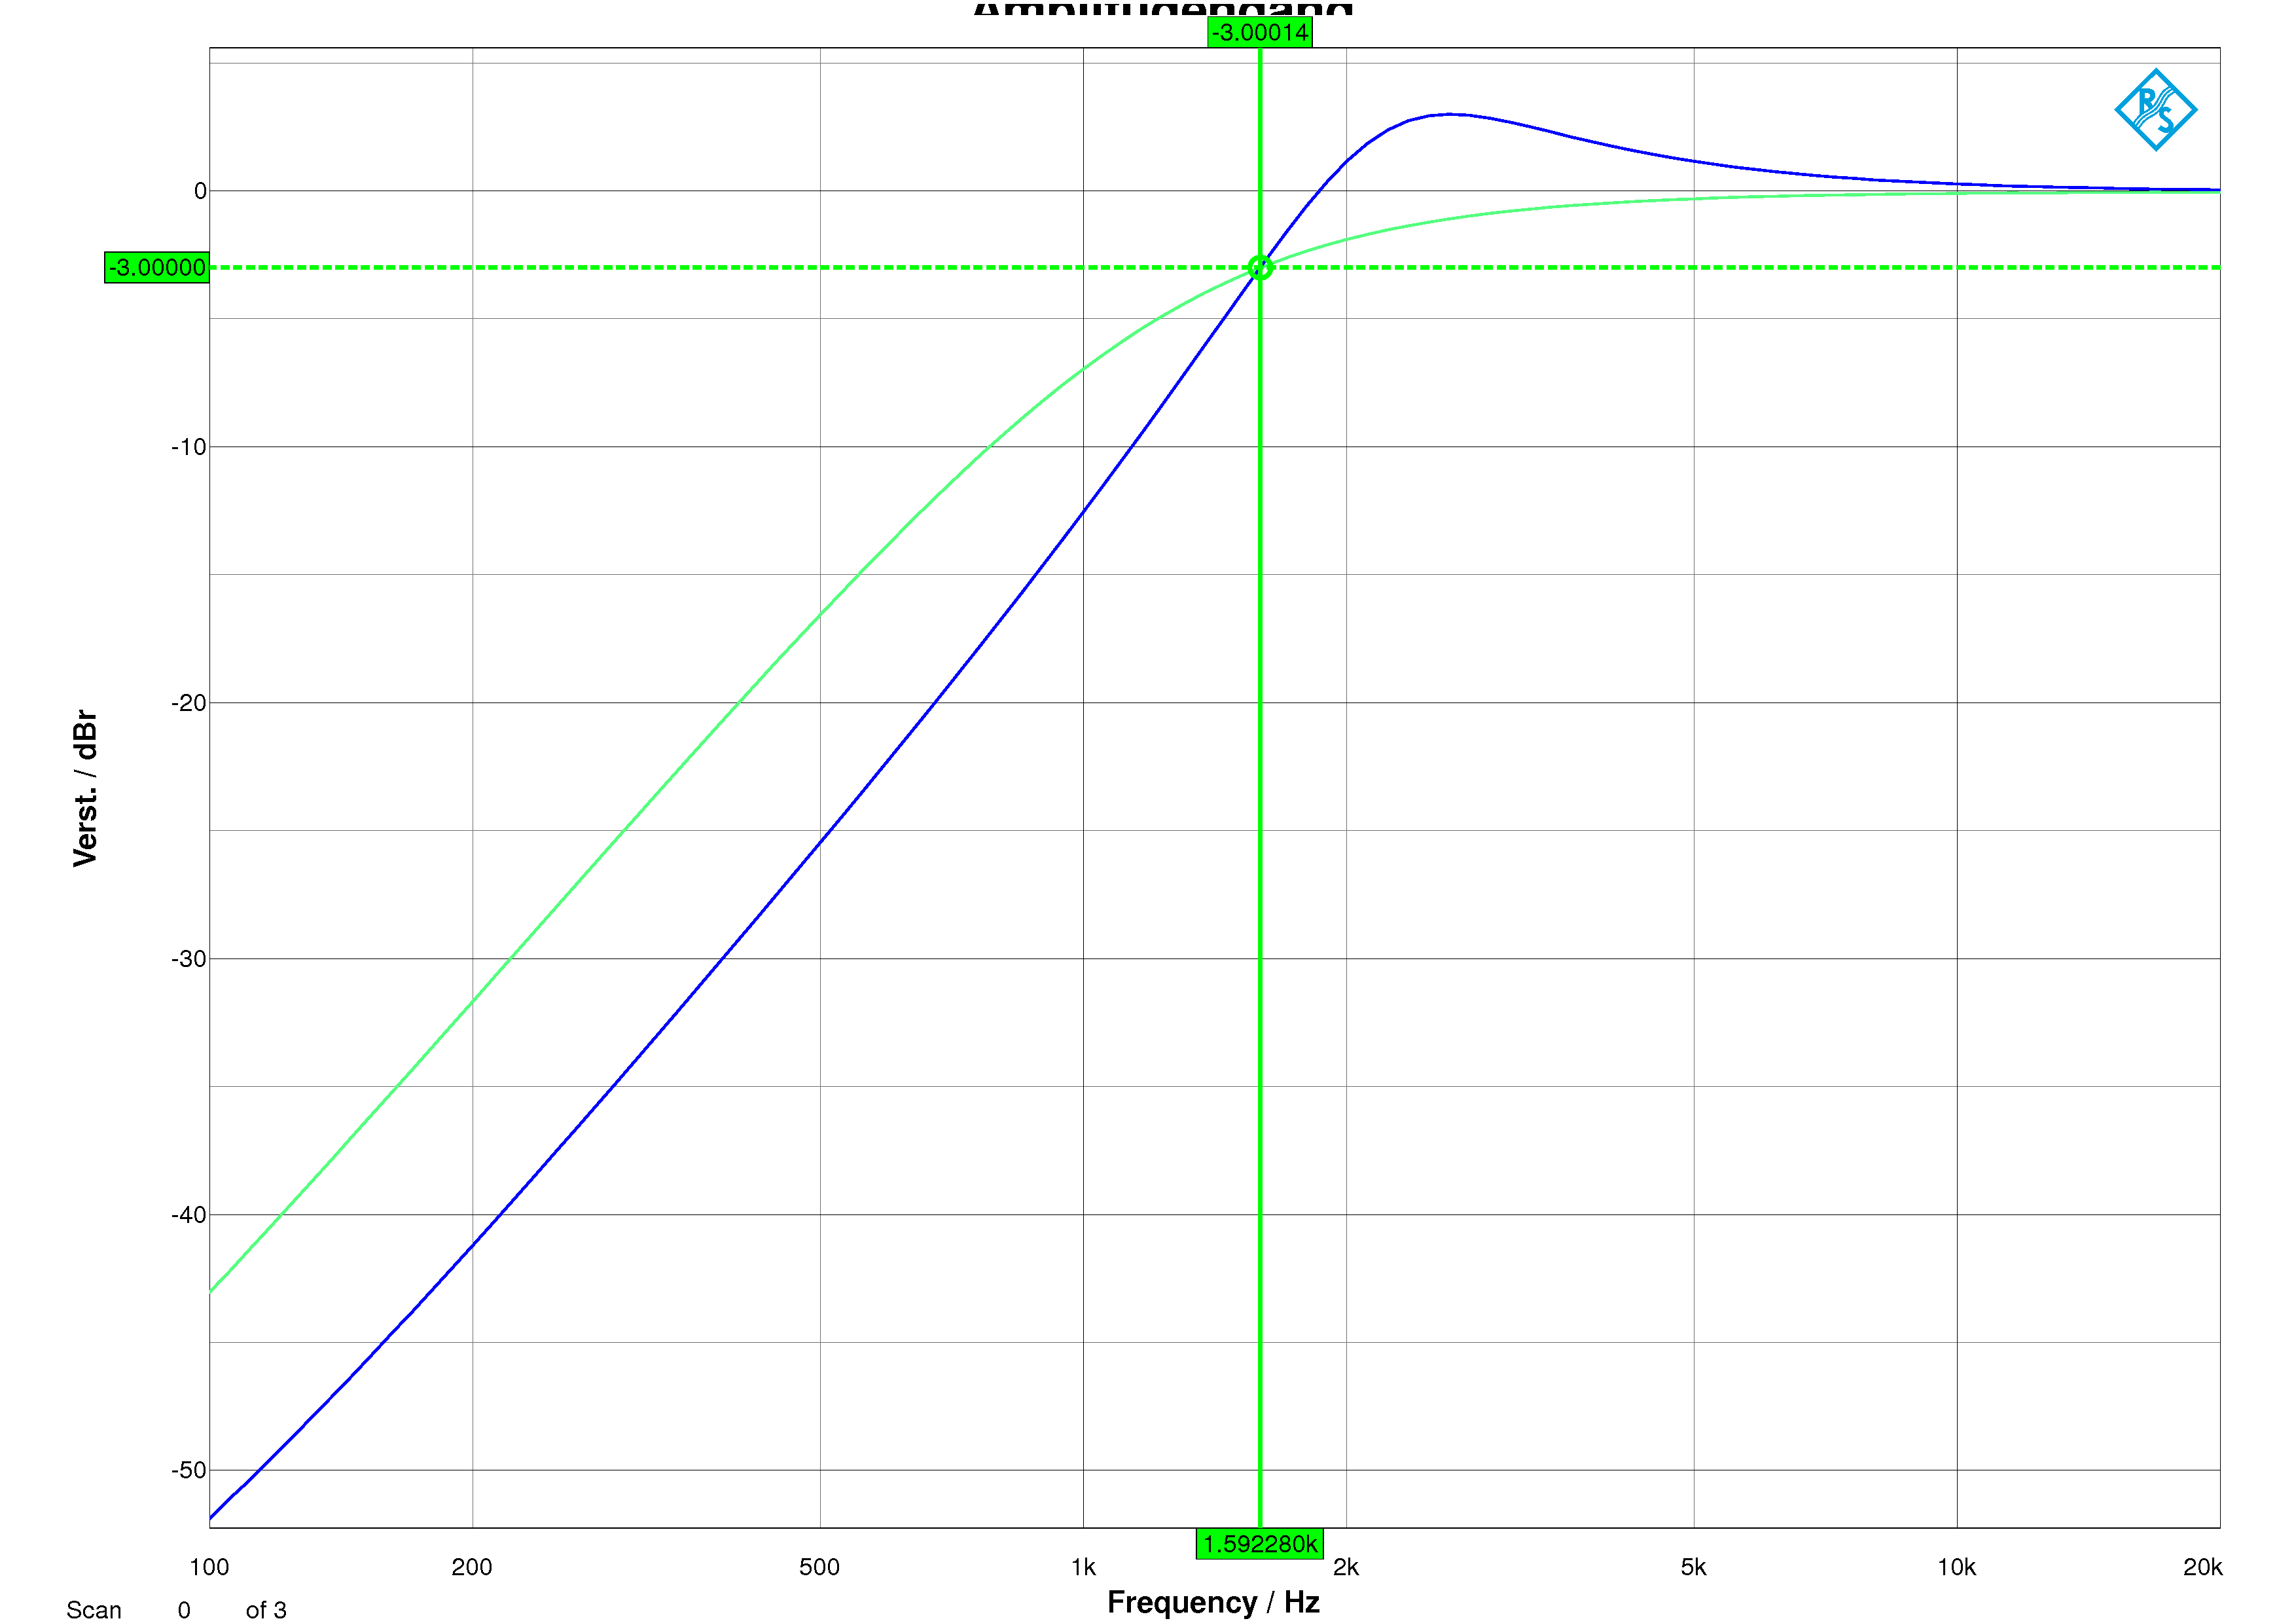
\includegraphics[width=0.60\linewidth]{Bilder/ImLabor/Amplitudengang_1_2_Tscheby_HP}
\caption{Amplitudengang Butterworth- und Tschebyscheff-Hochpass mit Marker bei Tschebyscheff}
\label{fig:Amplitudengang_1_2_Tscheby_HP}
\end{figure}

\begin{figure}[h]
\centering
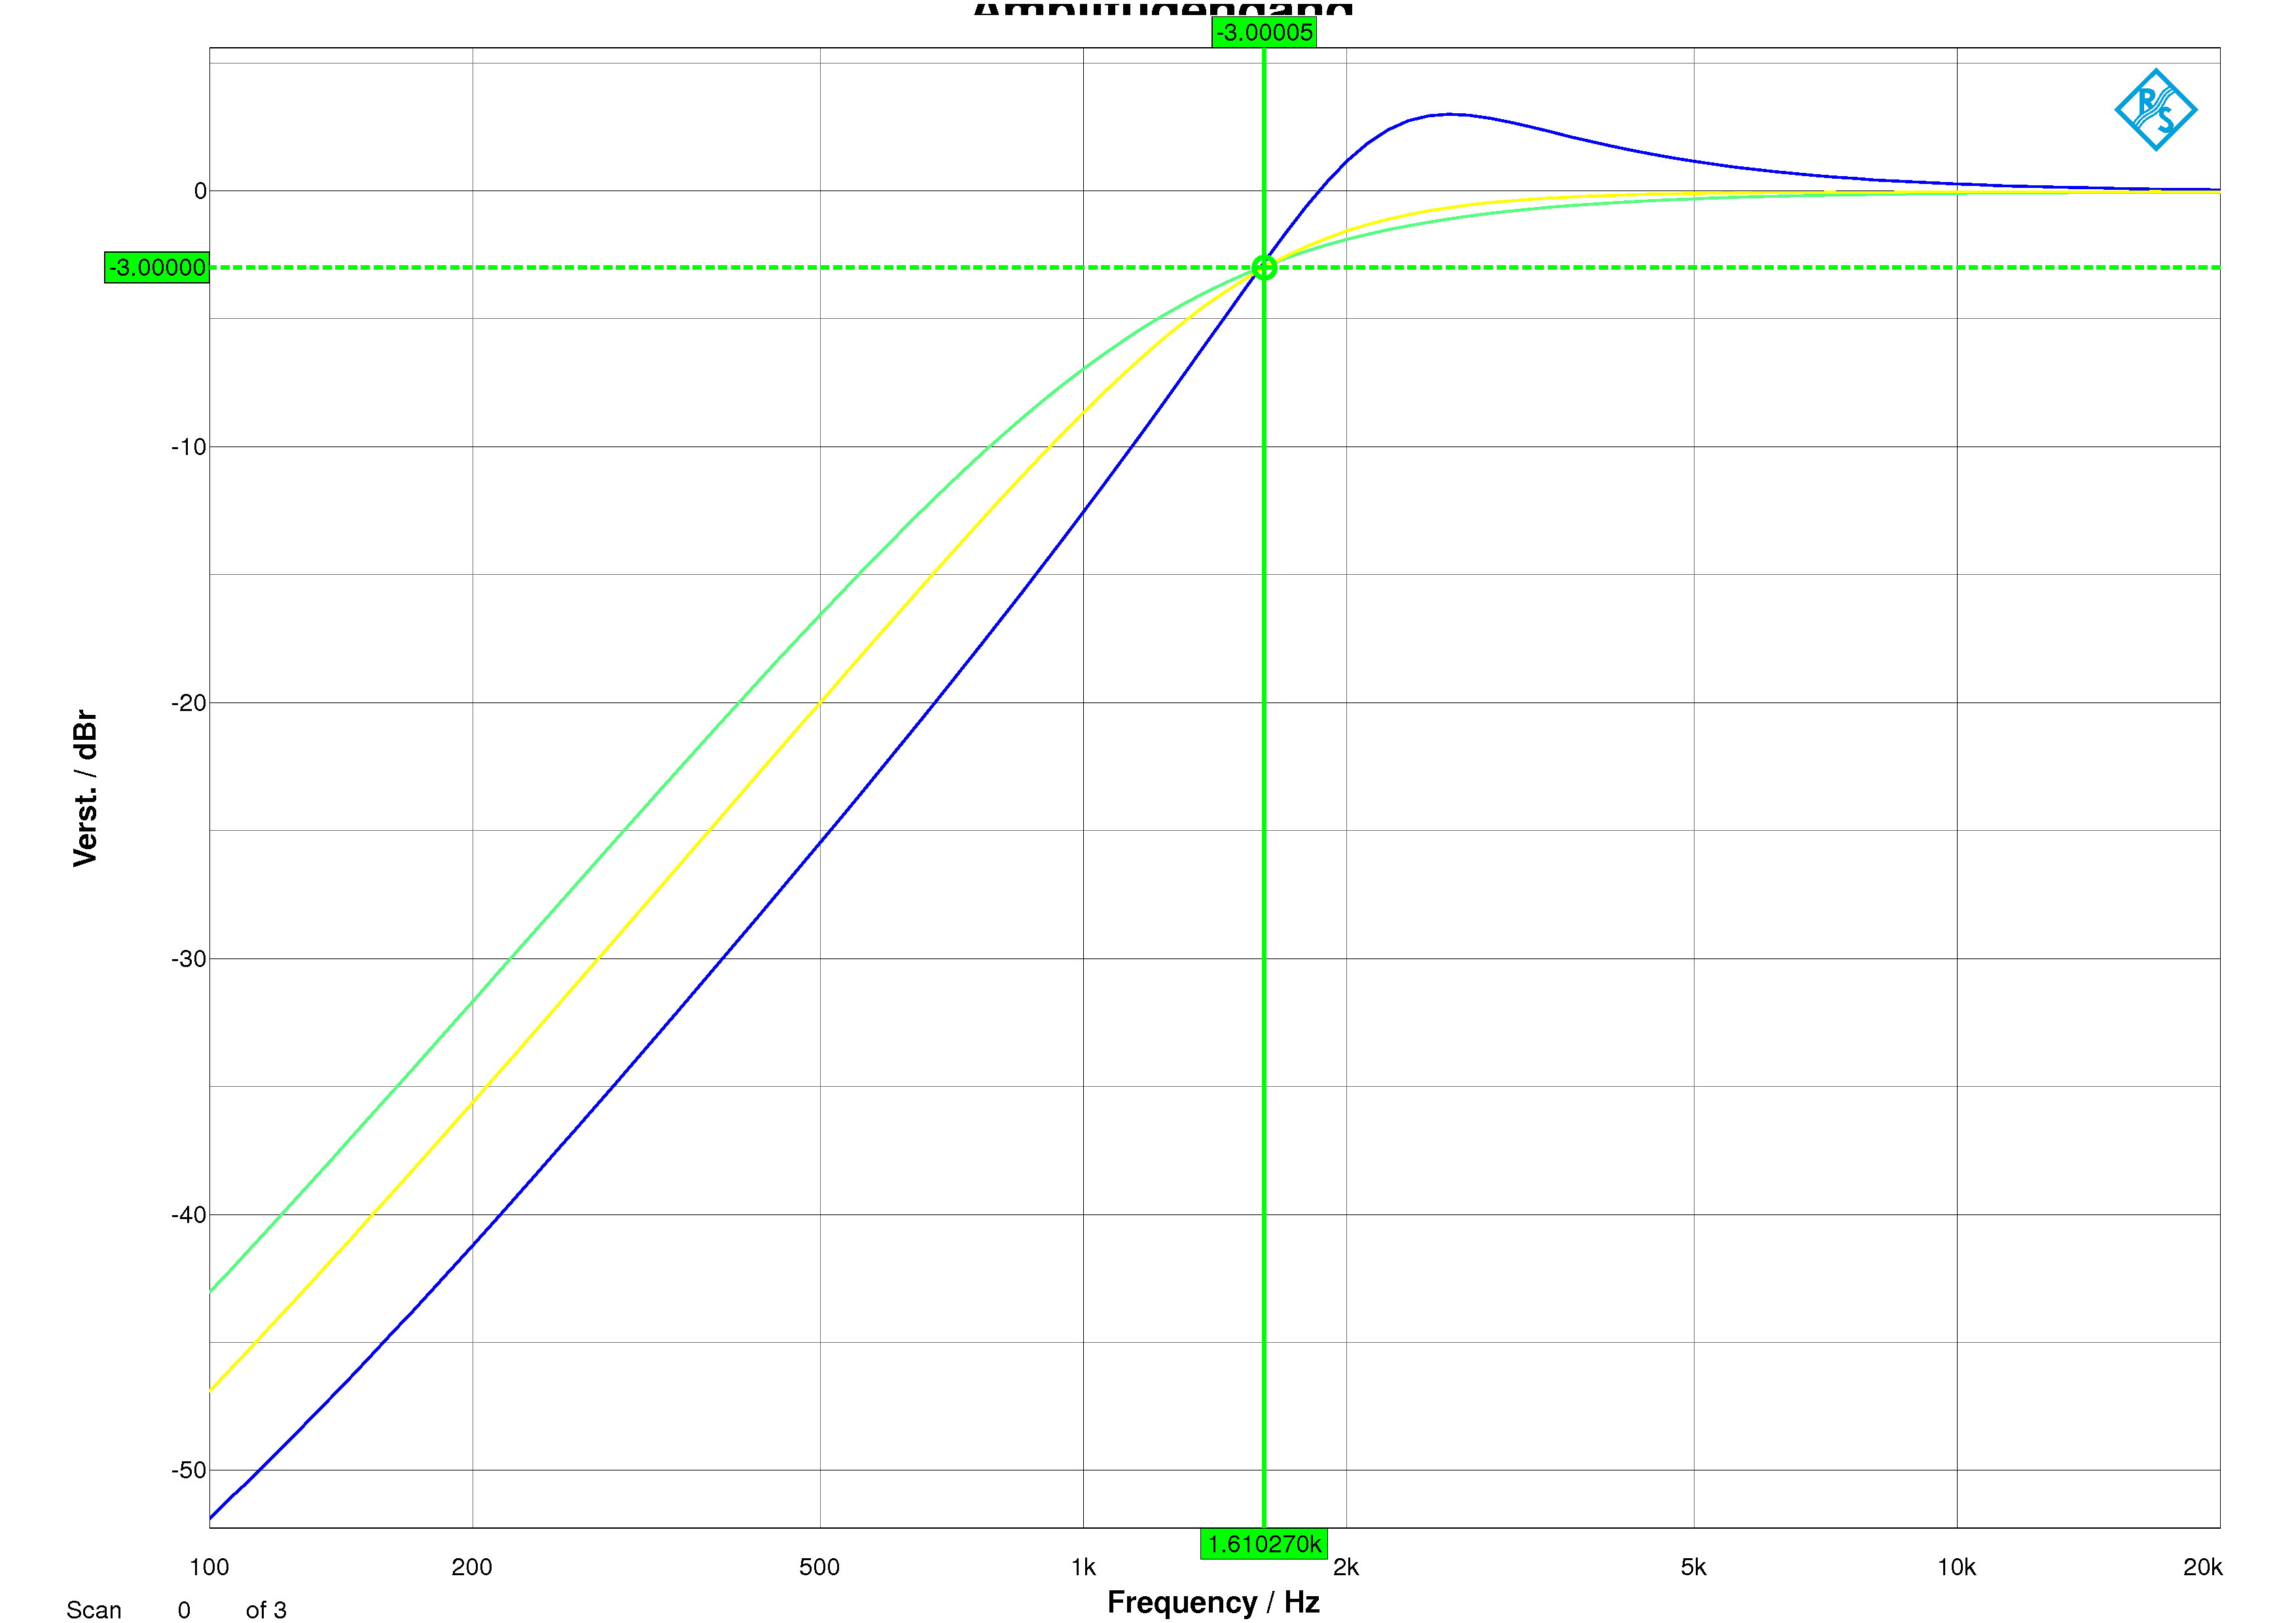
\includegraphics[width=0.60\linewidth]{Bilder/ImLabor/Amplitudengang_1_3_Bessel_HP_Alle}
\caption{Amplitudengang Butterworth-, Tschebyscheff- und Bessel-Hochpass mit Marker bei Bessel}
\label{fig:Amplitudengang_1_3_Bessel_HP_Alle}
\end{figure}

\newpage

\subsubsection{Bandpass/Bandsperre}
\begin{figure}[h]
\centering
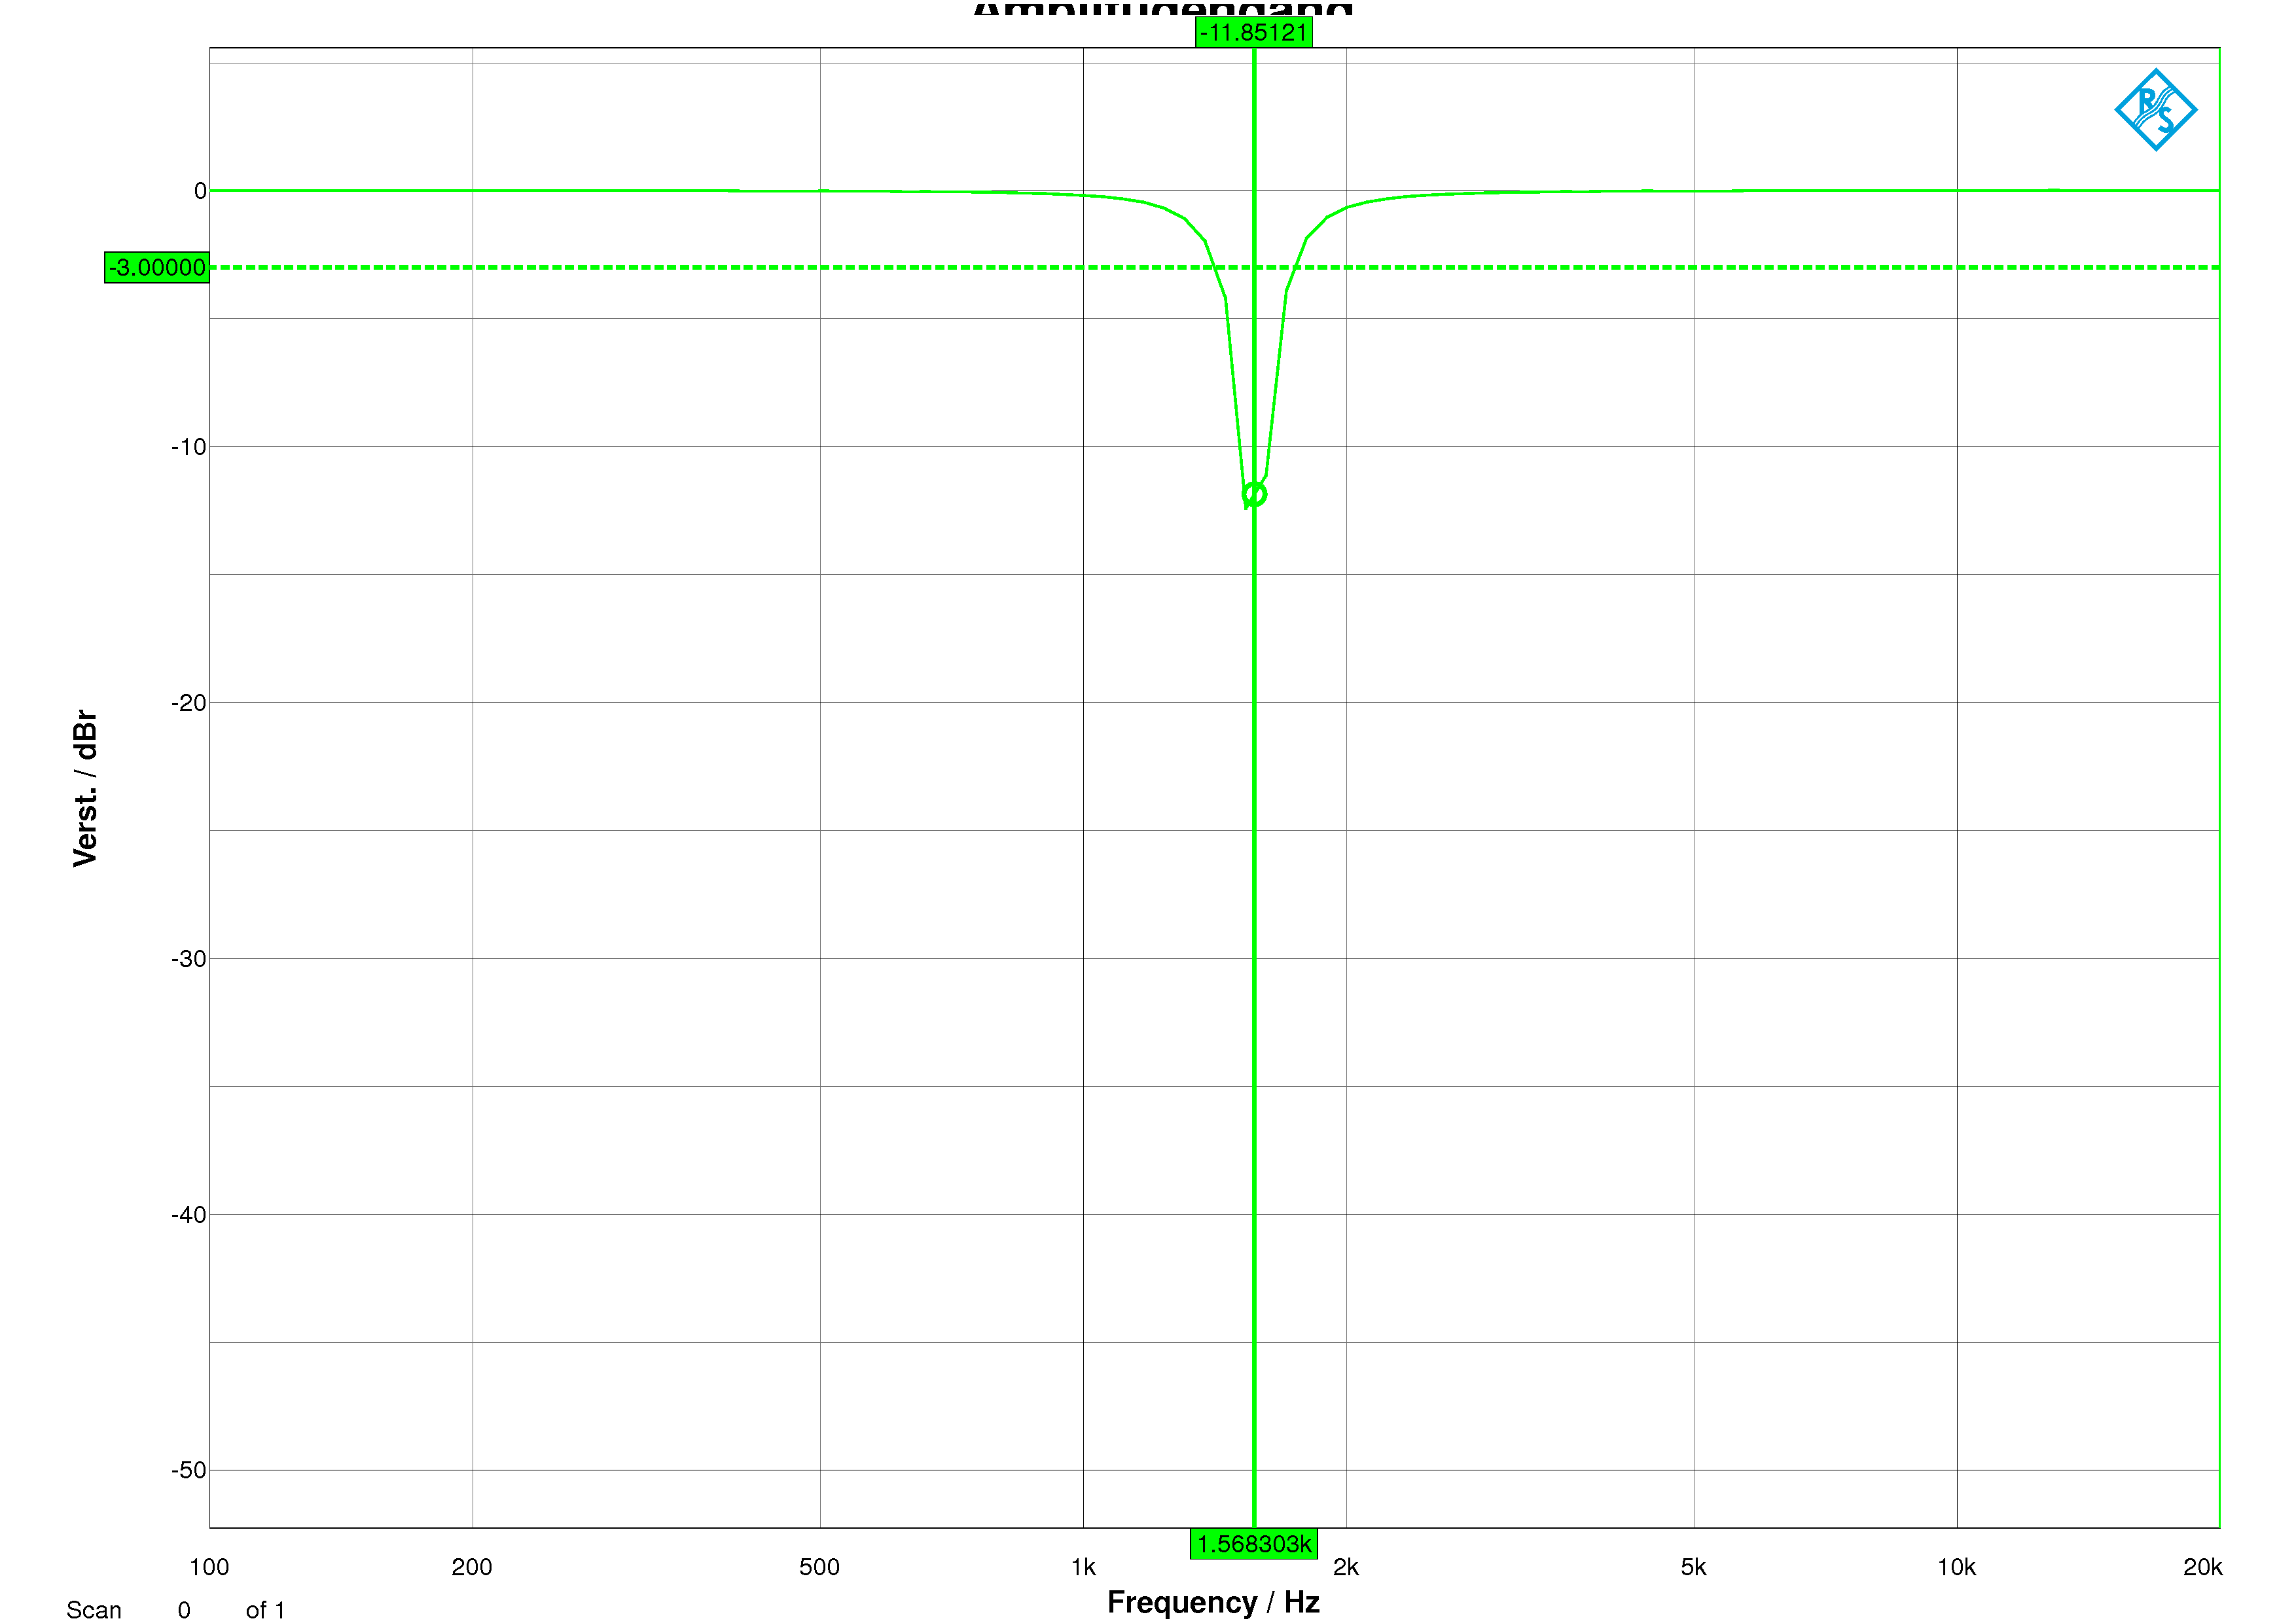
\includegraphics[width=0.60\linewidth]{Bilder/ImLabor/Amplitudengang_3_2_BS}
\caption{Amplitudengang Bandsperre mit Marker}
\label{fig:Amplitudengang_3_2_BS}
\end{figure}

\begin{figure}[h]
\centering
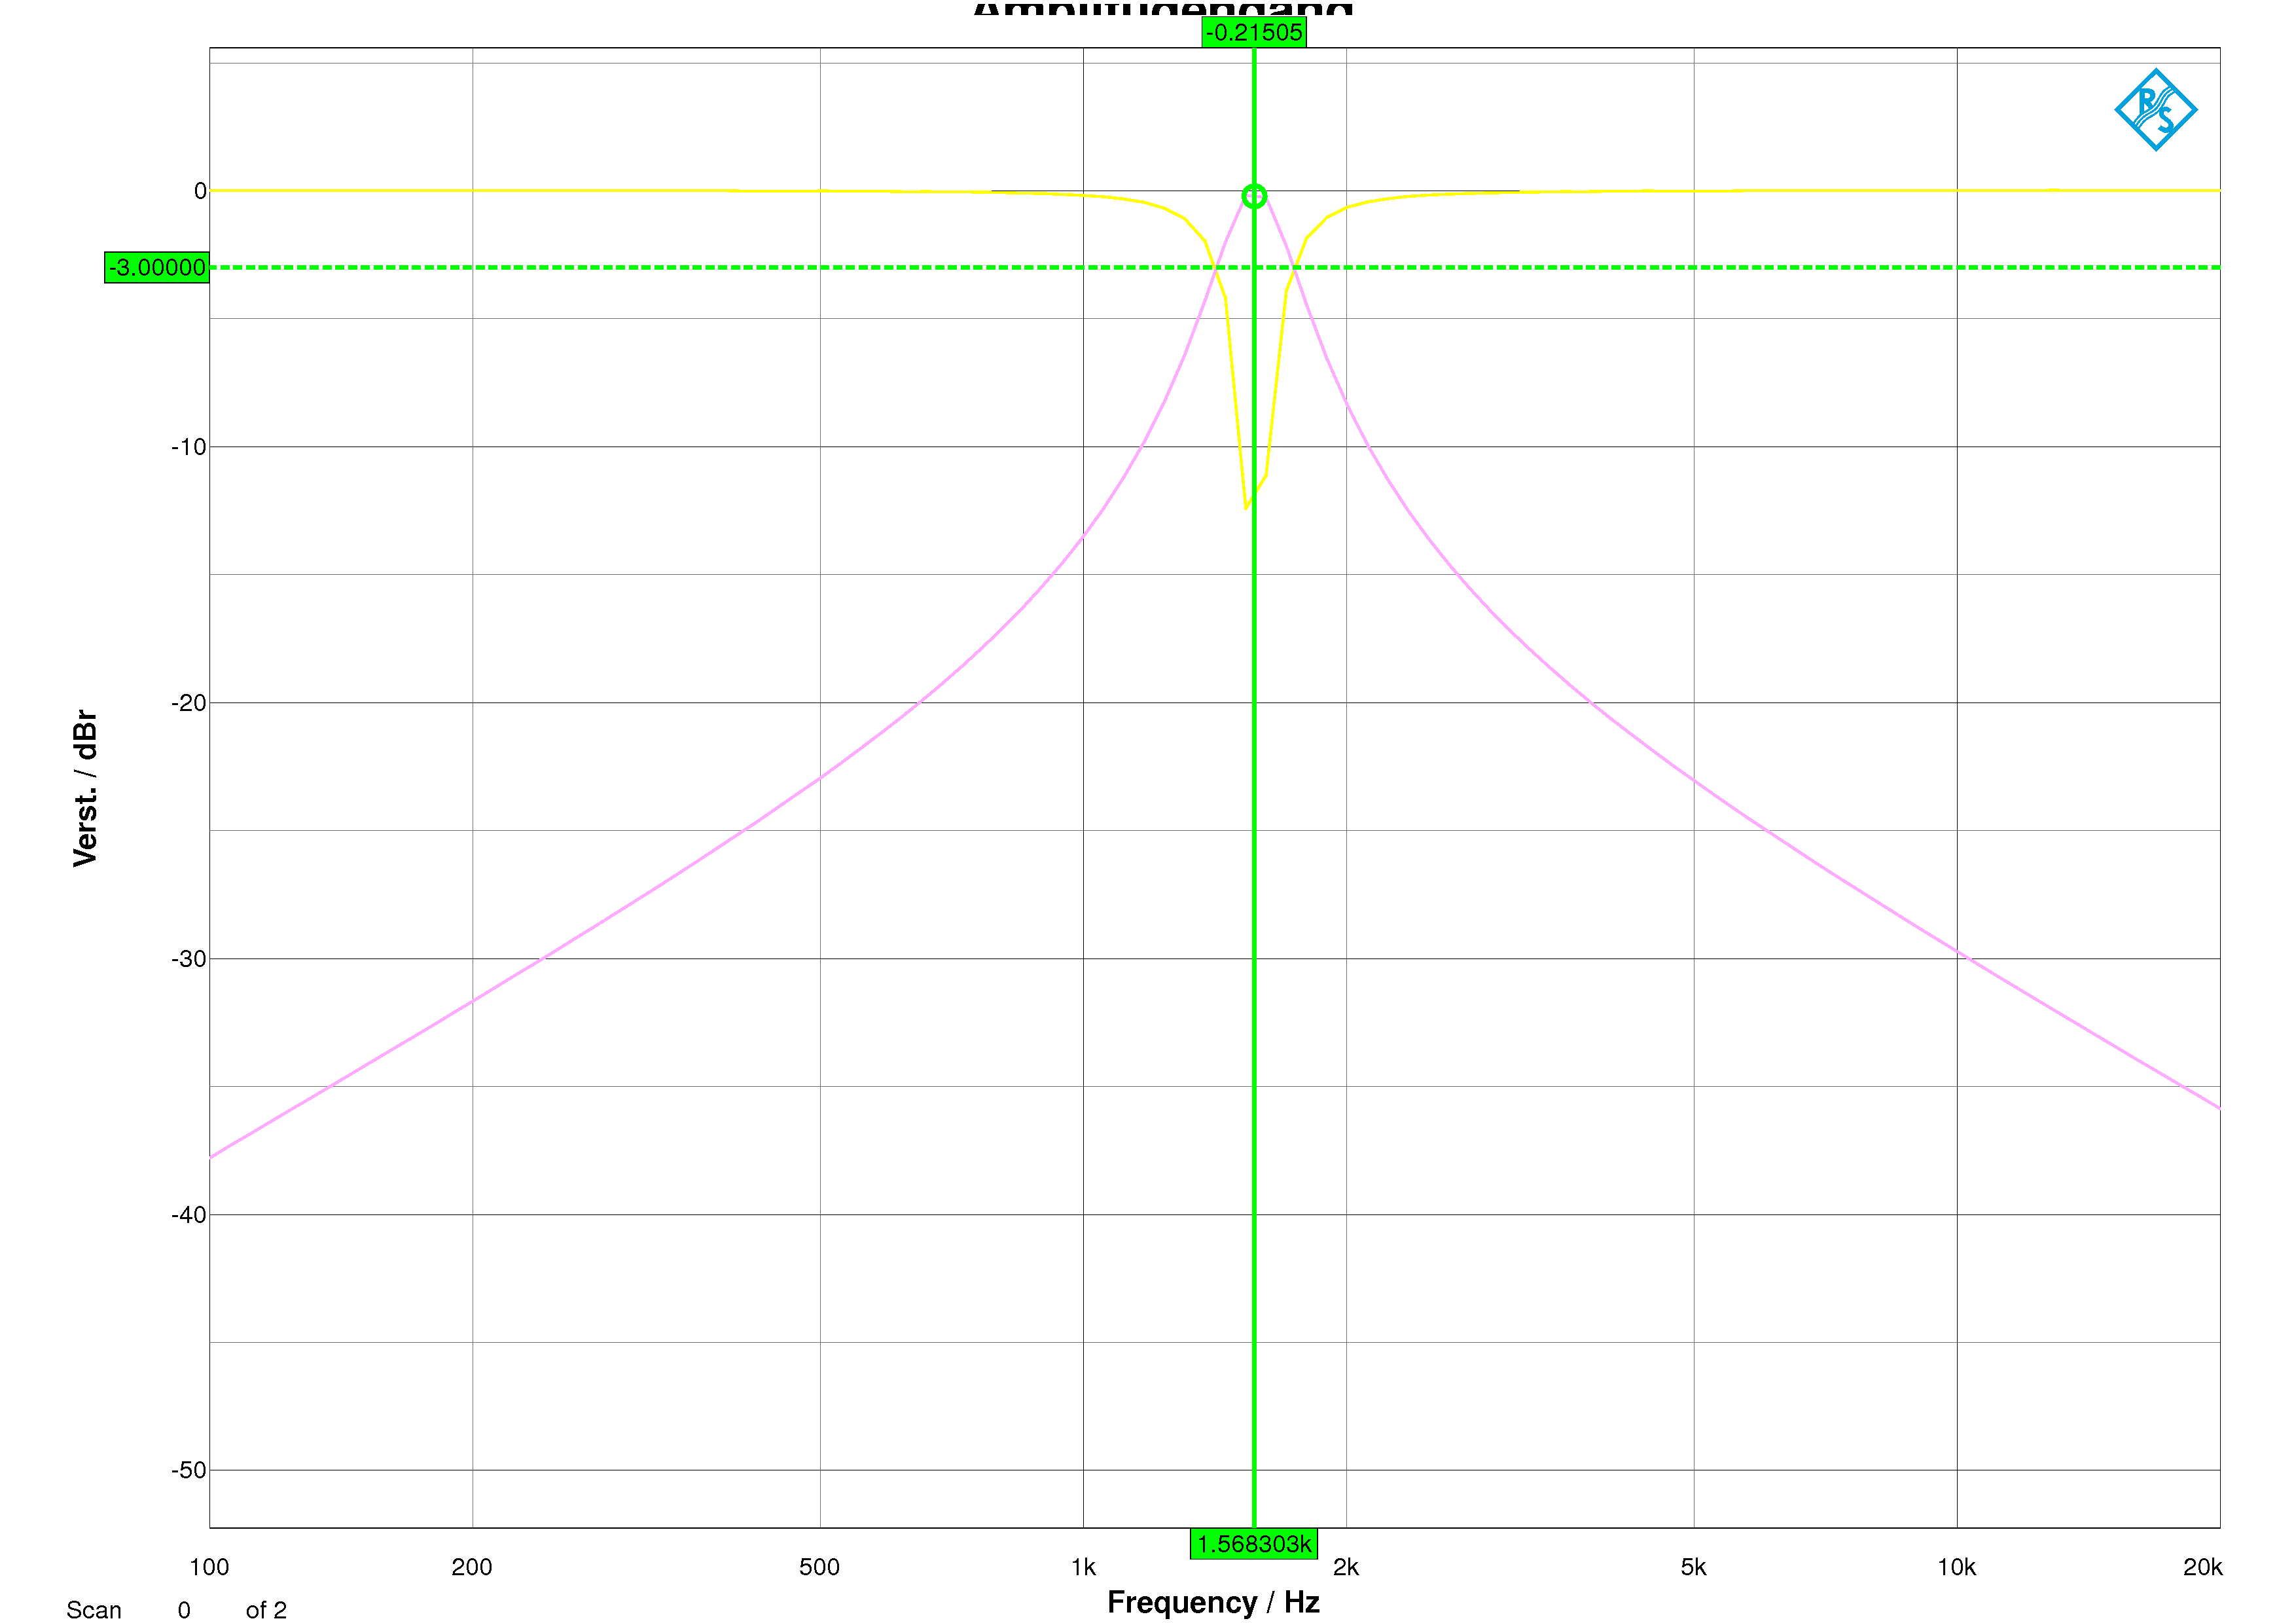
\includegraphics[width=0.60\linewidth]{Bilder/ImLabor/Amplitudengang_3_3_BP_BS}
\caption{Amplitudengang Bandsperre und Bandpass mit Maker beim Bandpass}
\label{fig:Amplitudengang_3_3_BP_BS}
\end{figure}

\newpage

\subsection{Phasengänge Tiefpässe}

\begin{figure}[h]
\centering
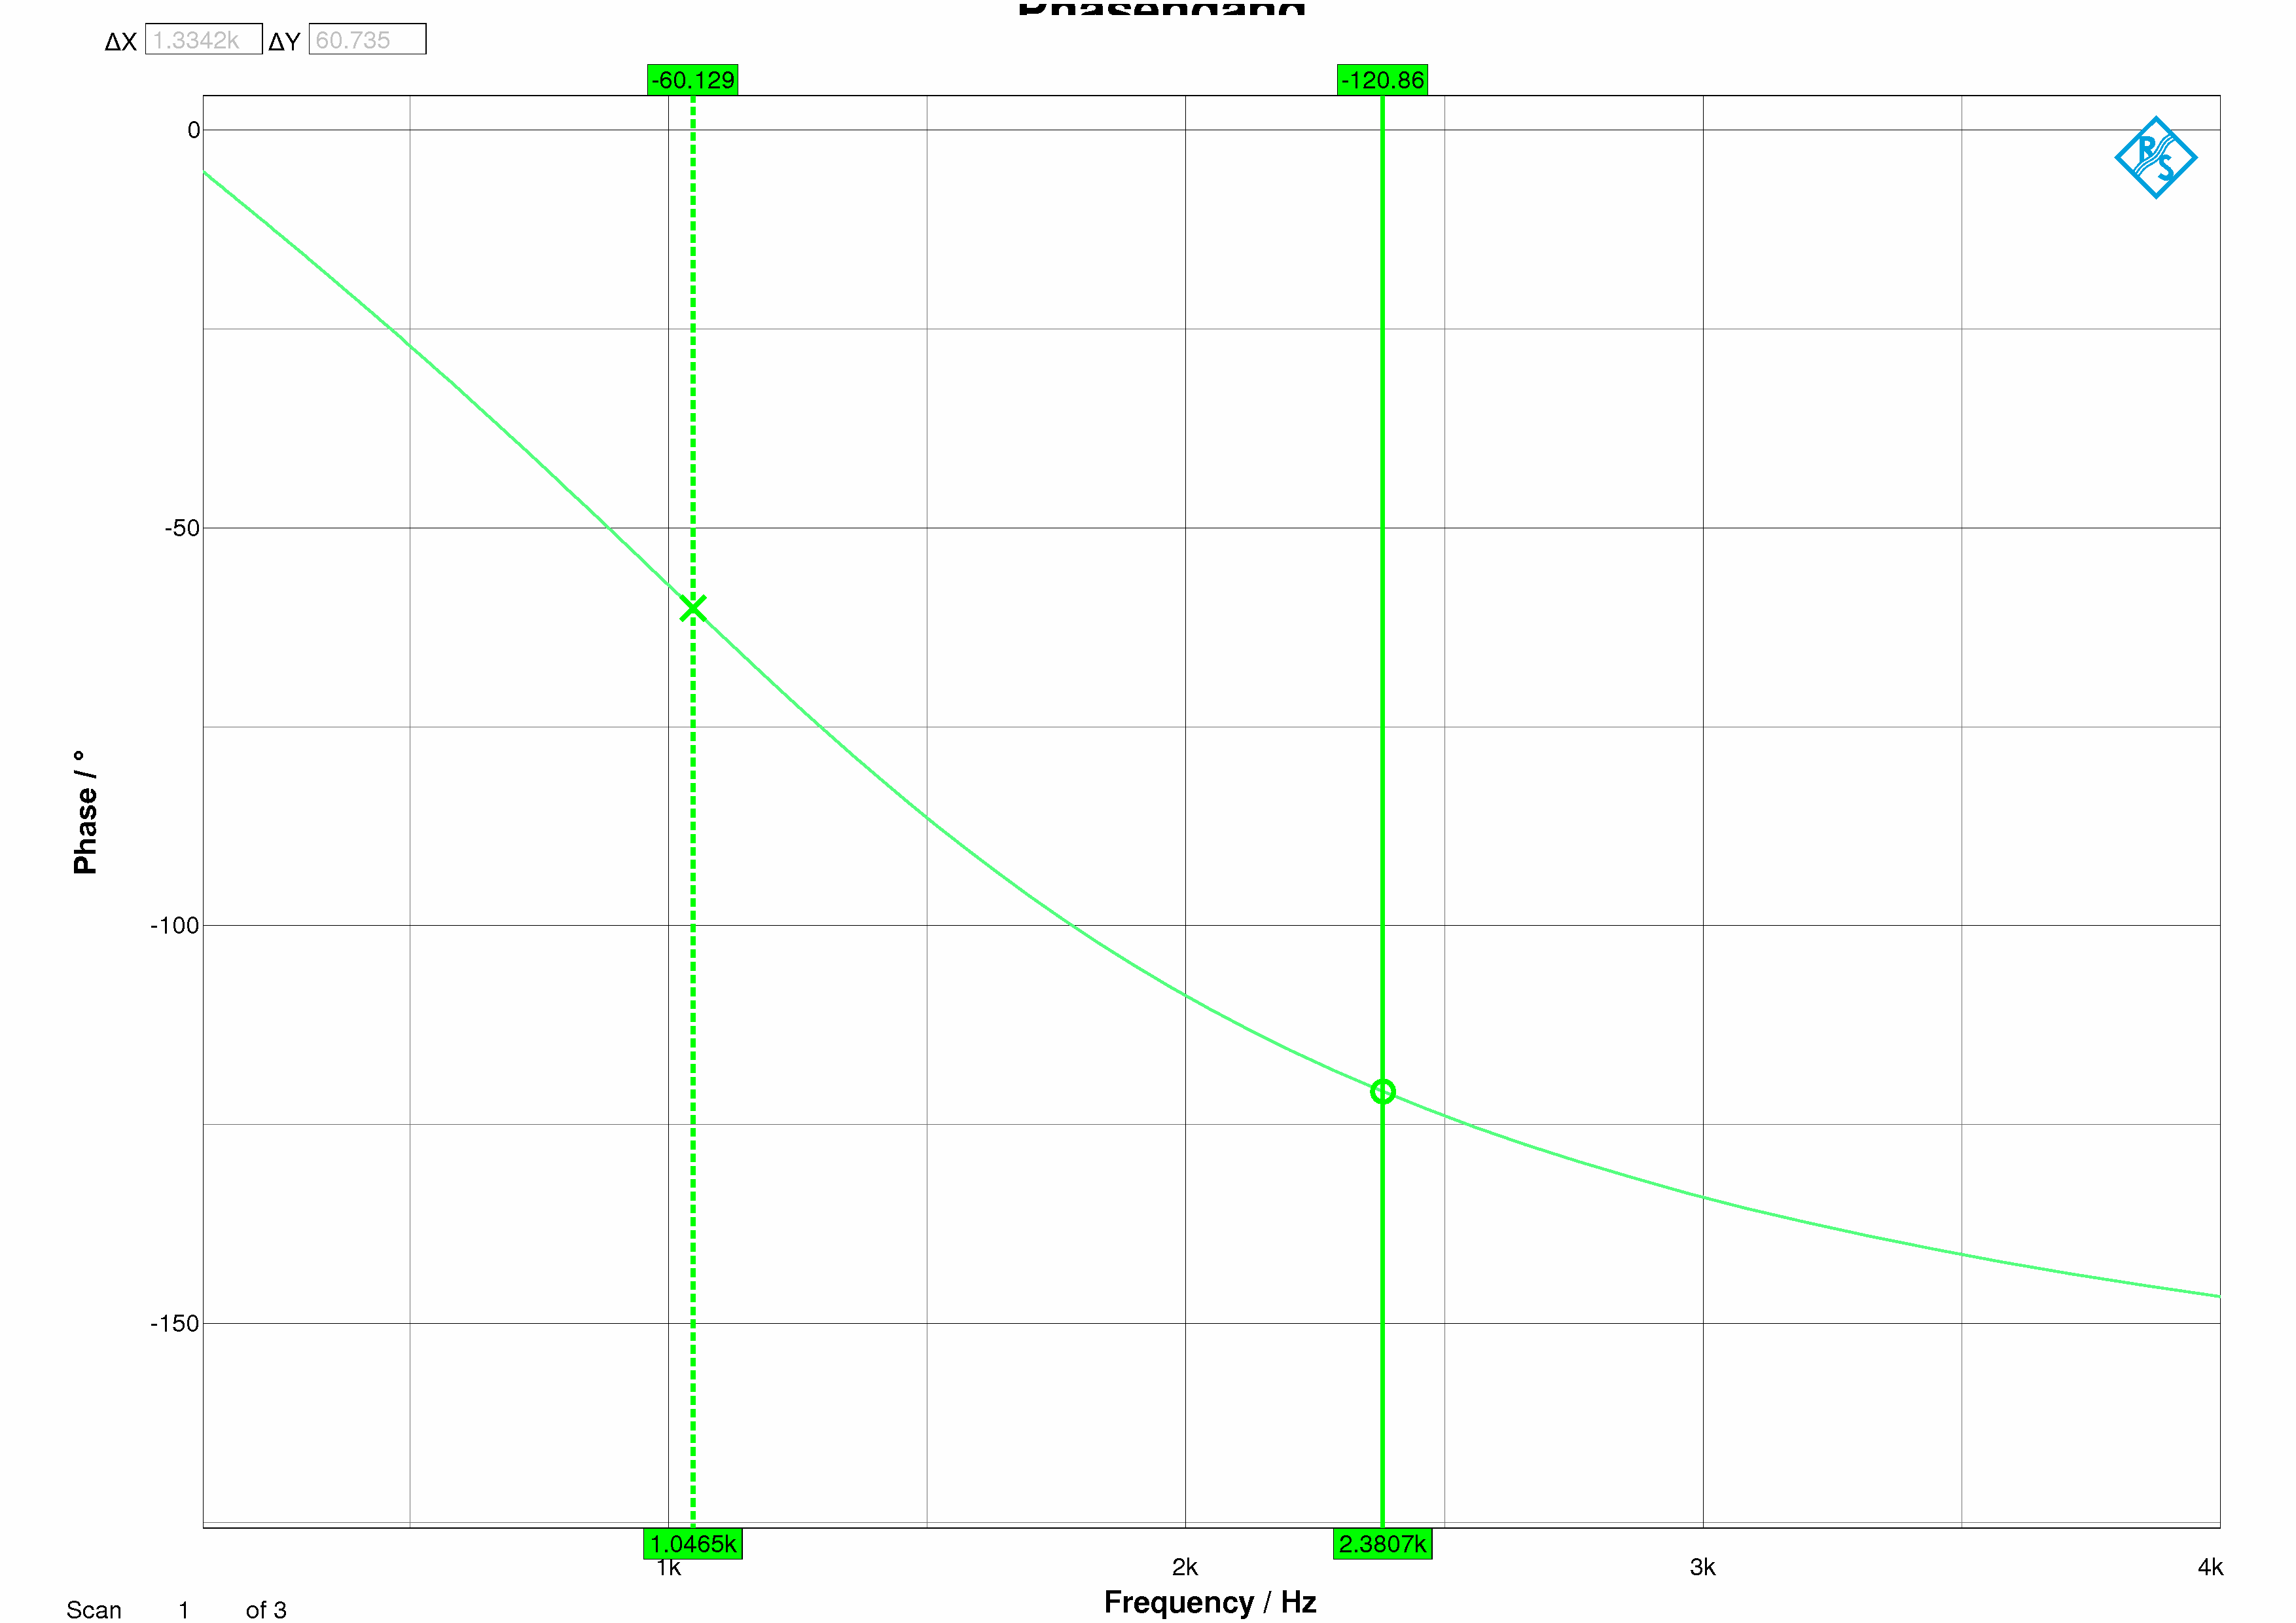
\includegraphics[width=0.60\linewidth]{Bilder/ImLabor/Phasengang_4_1_Butter_TP}
\caption{Phasengang Butterworth-Tiefpass mit Markern}
\label{fig:Phasengang_4_1_Butter_TP}
\end{figure}

\begin{figure}[h]
\centering
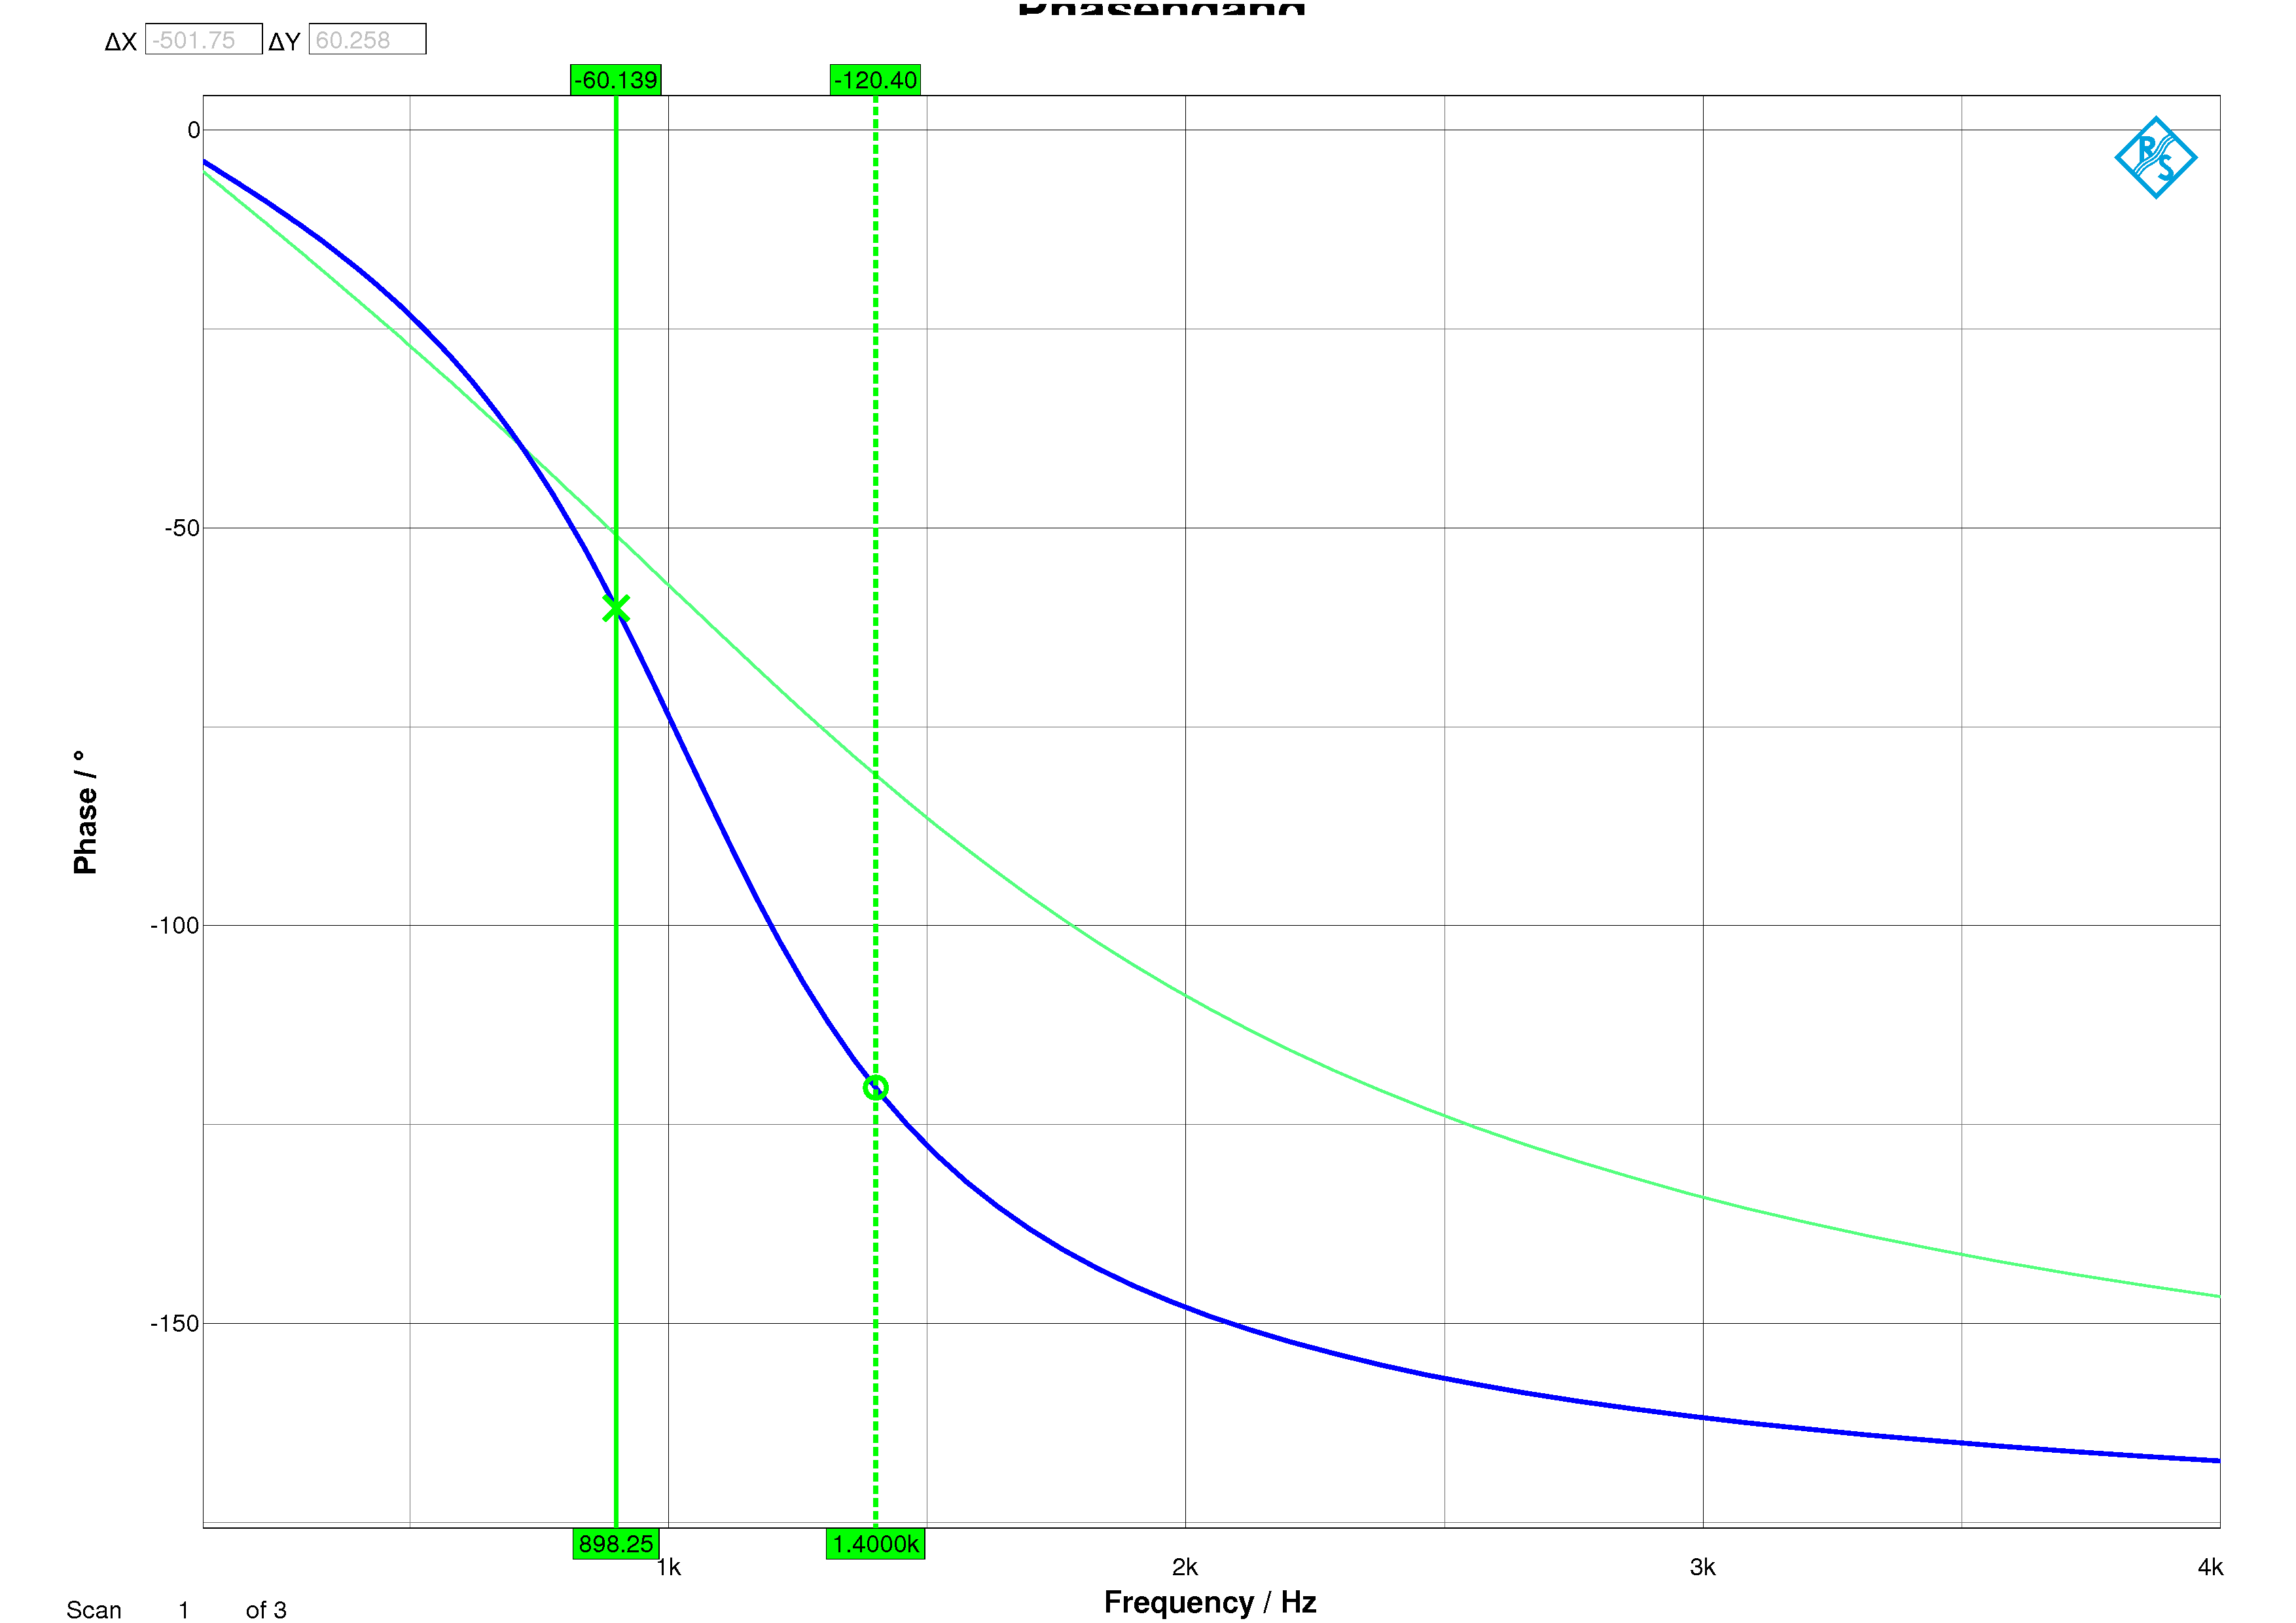
\includegraphics[width=0.60\linewidth]{Bilder/ImLabor/Phasengang_4_2_Tscheby_TP}
\caption{Phasengang Butterworth- und Tschebyscheff-Tiefpass mit Markern bei Tschebyscheff}
\label{fig:Phasengang_4_2_Tscheby_TP}
\end{figure}

\begin{figure}[h]
\centering
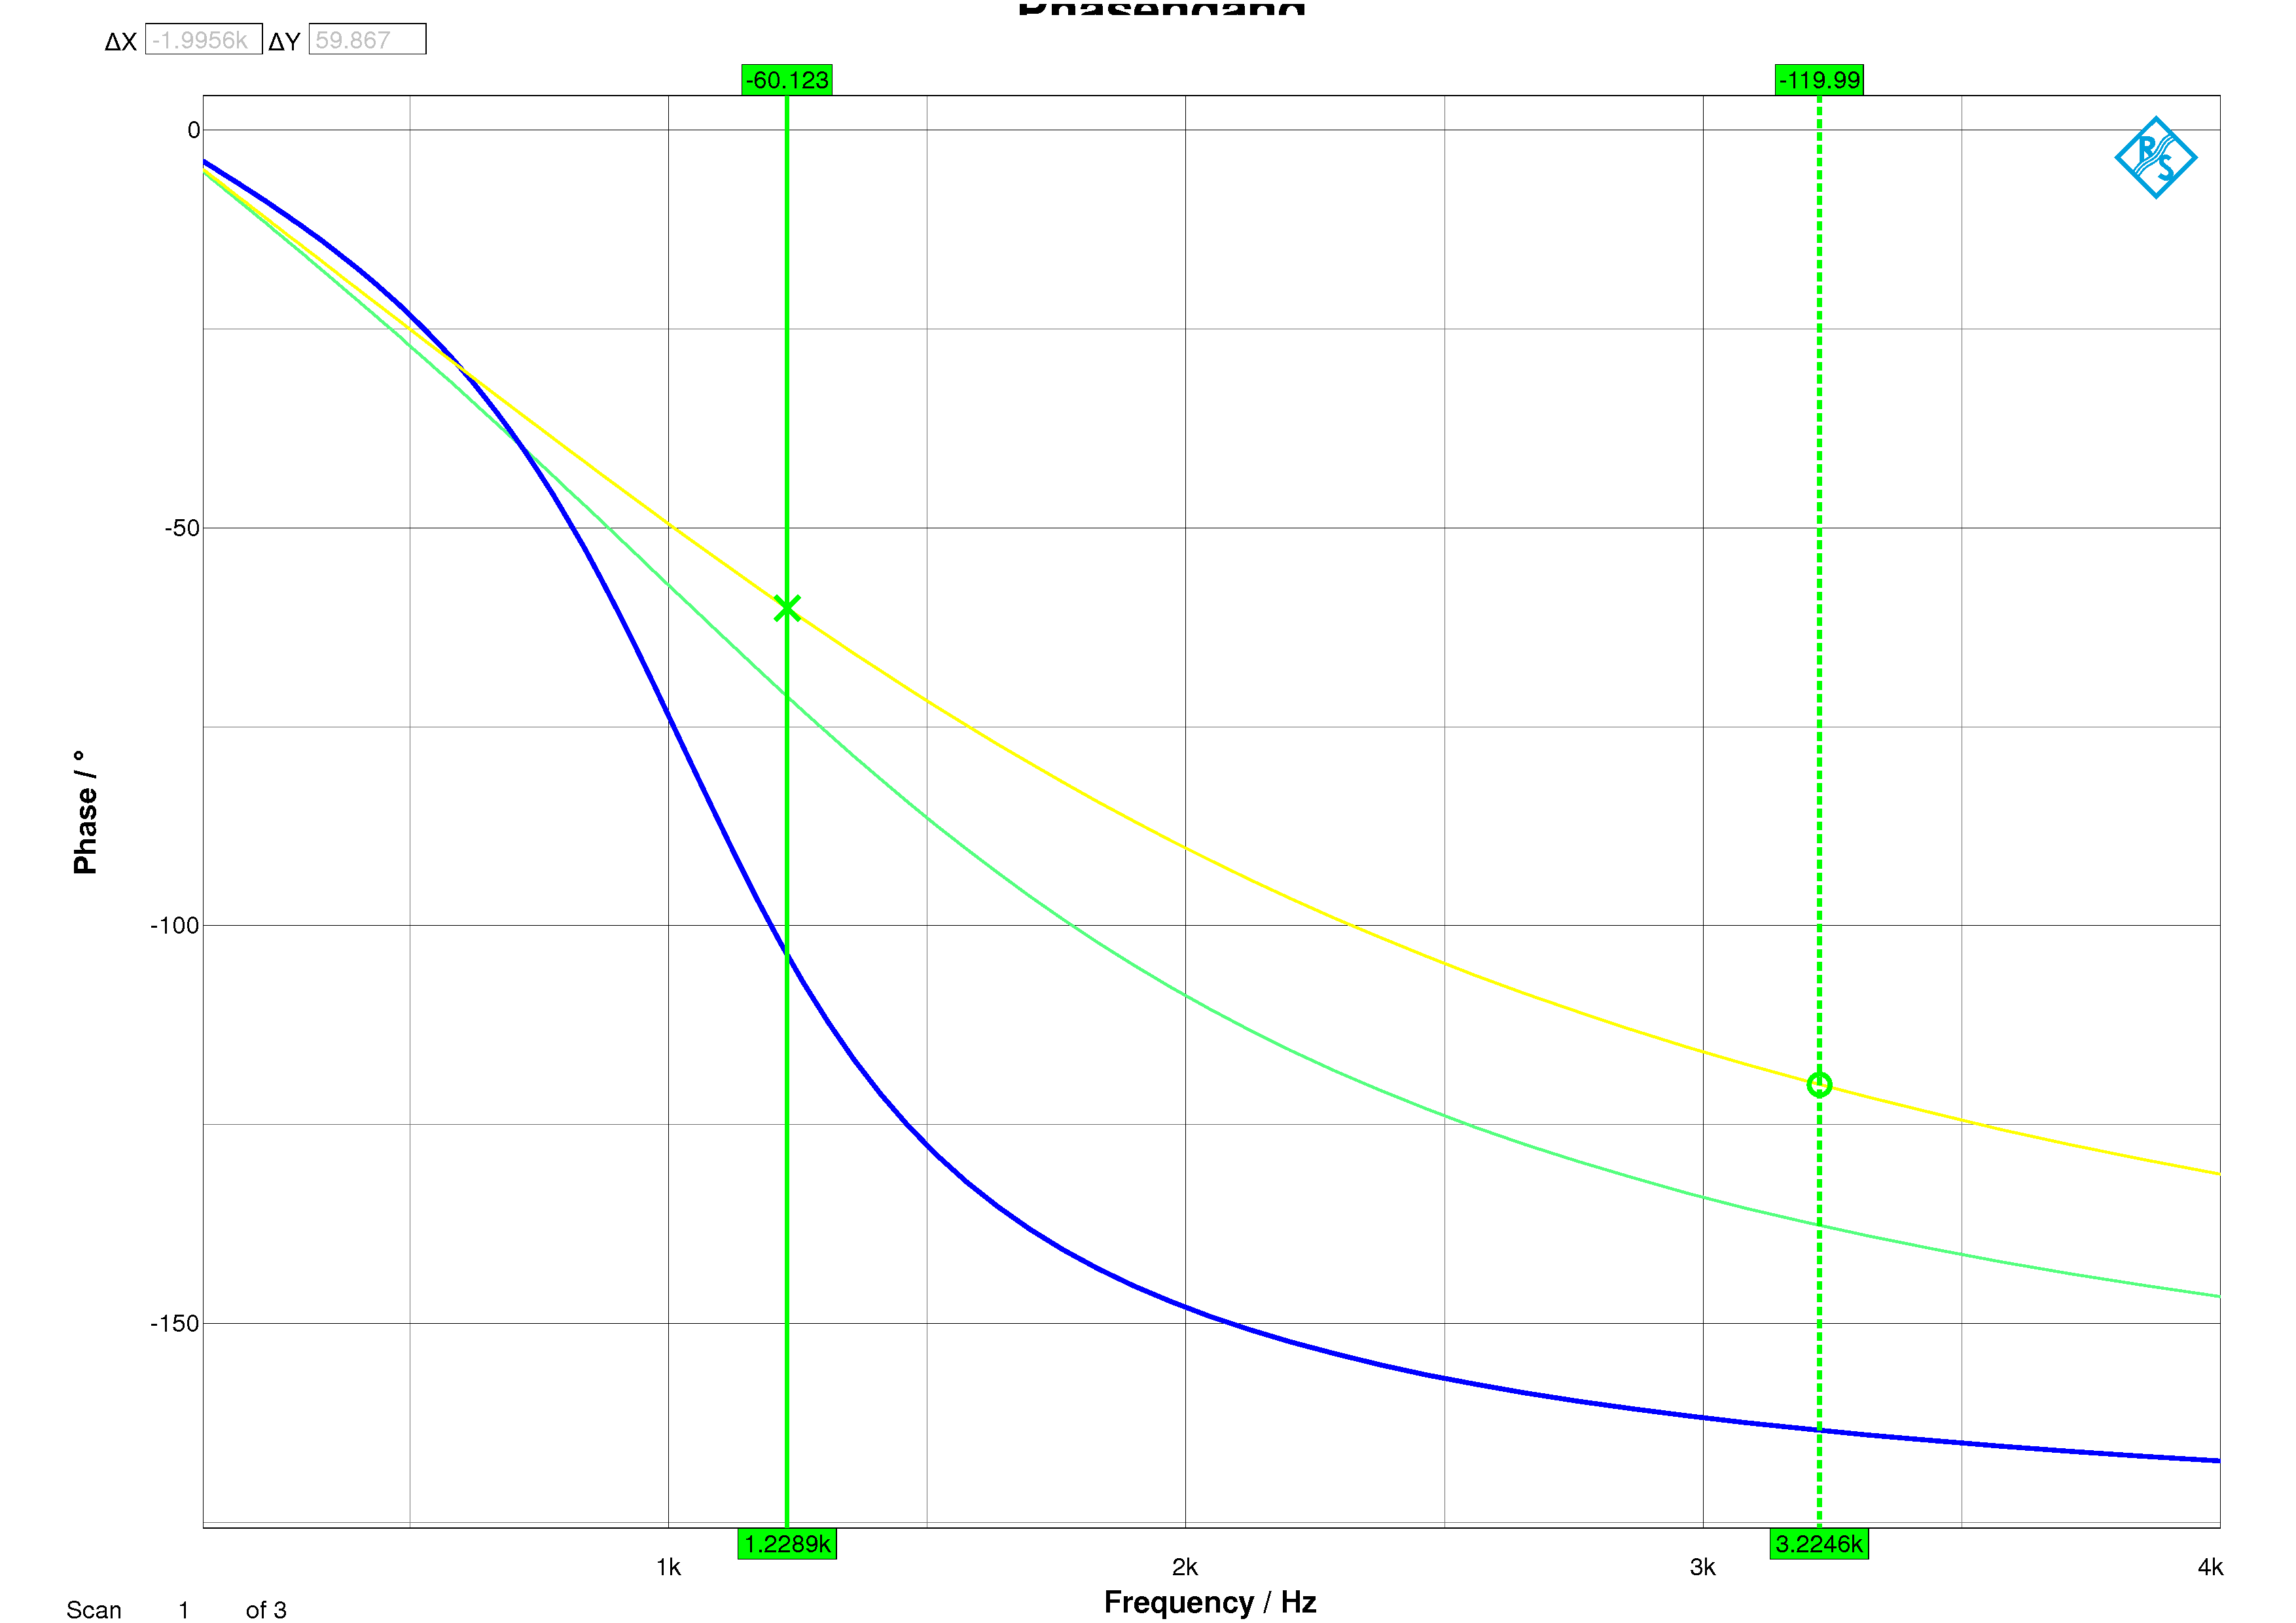
\includegraphics[width=0.60\linewidth]{Bilder/ImLabor/Phasengang_4_3_Bessel_TP_Alle}
\caption{Phasengang Butterworth-, Tschebyscheff- und Bessel-Tiefpass mit Markern bei Bessel}
\label{fig:Phasengang_4_3_Bessel_TP_Alle}
\end{figure}

\newpage

\subsection{Sprungantworten der Tiefpässe}
\subsubsection{Butterworth}

\begin{figure}[h]
	\centering
	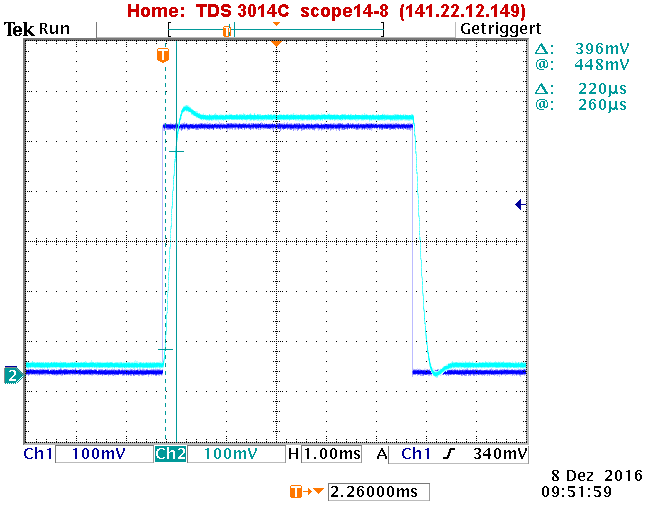
\includegraphics[width=0.60\linewidth]{Bilder/ImLabor/Sprungantwort_5_8_Butter_Anstiegszeit}
	\caption{Sprungantwort Butterworth: Messung der Anstiegszeit}
	\label{fig:Sprungantwort_5_8_Butter_Anstiegszeit_Anhang}
\end{figure}

\begin{figure}[h]
	\centering
	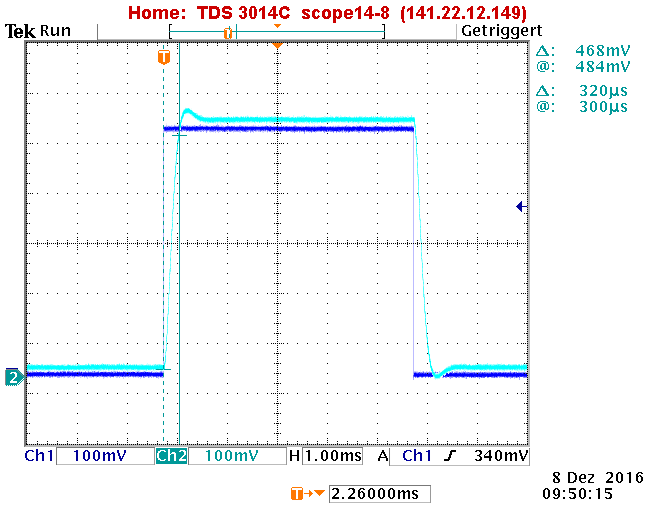
\includegraphics[width=0.60\linewidth]{Bilder/ImLabor/Sprungantwort_5_7_Butter_Einschwingzeit}
	\caption{Sprungantwort Butterworth: Messung der Einschwingzeit}
	\label{fig:Sprungantwort_5_7_Butter_Einschwingzeit}
\end{figure}

\begin{figure}[h]
	\centering
	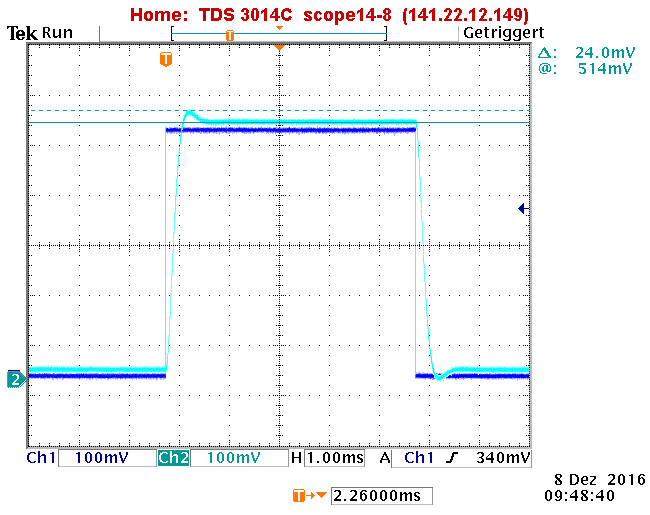
\includegraphics[width=0.60\linewidth]{Bilder/ImLabor/Sprungantwort_5_6_Butter_Ueberschwinger}
	\caption{Sprungantwort Butterworth: Messung des Überschwingers}
	\label{fig:Sprungantwort_5_6_Butter_Ueberschwinger}
\end{figure}

\newpage

\subsubsection{Tschebyscheff}

\begin{figure}[h]
	\centering
	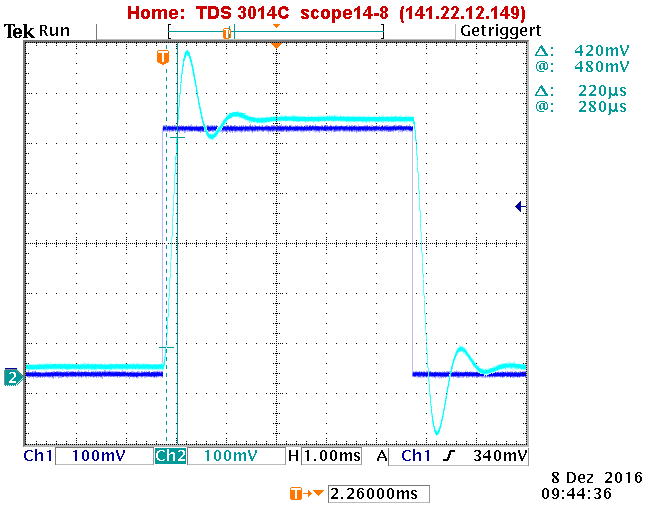
\includegraphics[width=0.60\linewidth]{Bilder/ImLabor/Sprungantwort_5_3_Tscheby_Anstiegszeit}
	\caption{Sprungantwort Tschebyscheff: Messung der Anstiegszeit}
	\label{fig:Sprungantwort_5_3_Tscheby_Anstiegszeit_Anhang}
\end{figure}

\begin{figure}[h]
	\centering
	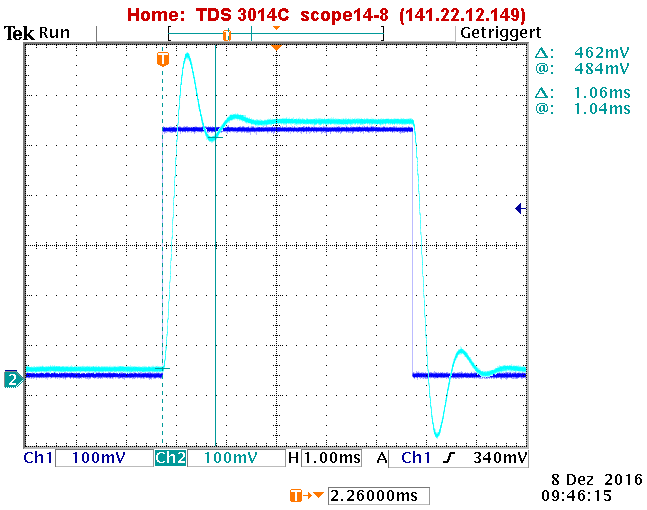
\includegraphics[width=0.60\linewidth]{Bilder/ImLabor/Sprungantwort_5_4_Tscheby_Einschwingzeit}
	\caption{Sprungantwort Tschebyscheff: Messung der Einschwingzeit}
	\label{fig:Sprungantwort_5_4_Tscheby_Einschwingzeit}
\end{figure}

\begin{figure}[h]
\centering
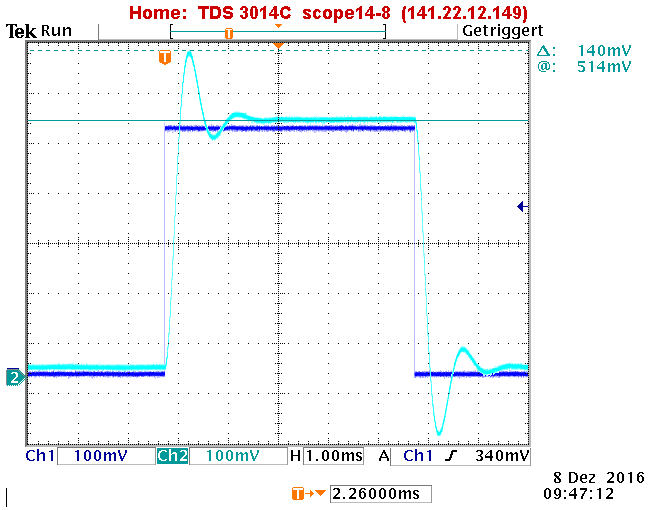
\includegraphics[width=0.60\linewidth]{Bilder/ImLabor/Sprungantwort_5_5_Tscheby_Ueberschwinger}
\caption{Sprungantwort Tschebyscheff: Messung des Überschwingers}
\label{fig:Sprungantwort_5_5_Tscheby_Ueberschwinger}
\end{figure}

\newpage

\subsubsection{Bessel}

\begin{figure}[h]
\centering
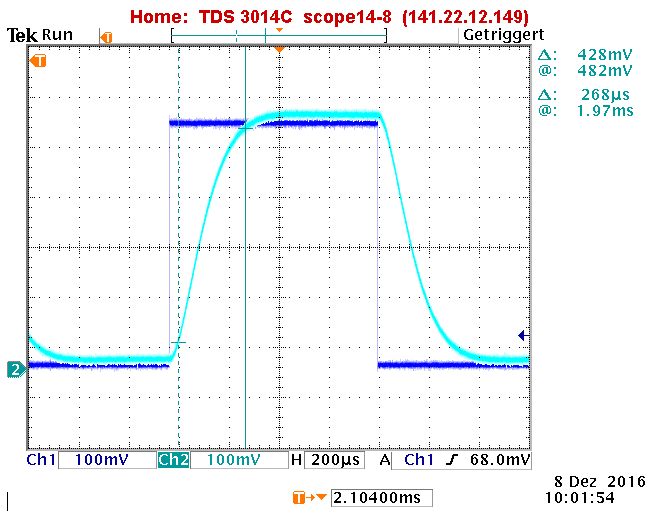
\includegraphics[width=0.60\linewidth]{Bilder/ImLabor/Sprungantwort_5_1_Bessel_Anstiegszeit}
\caption{Sprungantwort Bessel: Messung der Anstiegszeit}
\label{fig:Sprungantwort_5_1_Bessel_Anstiegszeit_Anhang}
\end{figure}

\begin{figure}[h]
\centering
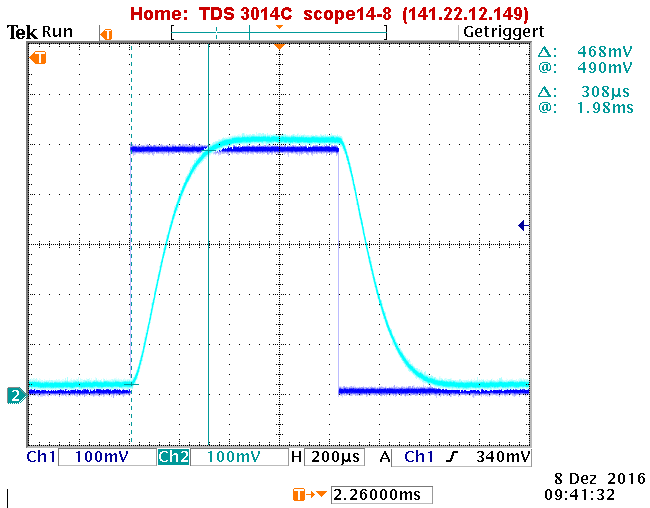
\includegraphics[width=0.60\linewidth]{Bilder/ImLabor/Sprungantwort_5_2_Bessel_Einschwingzeit}
\caption{Sprungantwort Bessel: Messung der Einschwingzeit}
\label{fig:Sprungantwort_5_2_Bessel_Einschwingzeit}
\end{figure}

















	
%	\bibliography{bibfile}{}
%	\bibliographystyle{plain}
	
	
\end{document}